\documentclass[a4paper,12pt]{article}
% a4paper sets it up with the measures for A4 paper
% 12pt is the lettering size, (you can use 11pt or 12pt)

% this produces A4 pages with a lot more text on each page
\usepackage{a4wide}

% this tells LaTeX how the latex file is encoded
% on a modern linux usually utf8, older linux in Sweden usually latin1
% Windows has sometimes, but not always, its own encoding
% latin1 and utf8 allow direct input of accented characters like åäö 

% uncomment (i.e. remove the % in front) for a fancier bibliography
%\bibliographystyle{natbib}

% this defines the \includegraphics command used for including figures
\usepackage{graphicx}

% the amsmath package has a lot of useful stuff for equations,
% especially for ligning up multiple equations
\usepackage{amsmath}

\usepackage{feynmp}
\DeclareGraphicsRule{*}{mps}{*}{}

\usepackage{braket}

%useful for dealing with labels, uncomment while writing
%\usepackage{showkeys}

\renewcommand{\theequation}{\thesection.\arabic{equation}}

% external packages 
\usepackage[utf8]{inputenc}

% package for figures
\usepackage{graphicx}
\usepackage{caption}
%\usepackage{subcaption}

% combine citations into a range
\usepackage{cite}

% ulem implements \sout{} for overstriking text
%\usepackage{ulem}

%% define page size
%\setlength{\textheight}{235mm}
%\setlength{\topmargin}{6mm}
%\setlength{\headheight}{0mm}
%\setlength{\headsep}{0mm}
%\setlength{\footskip}{15mm}
%\setlength{\textwidth}{163mm}
%\setlength{\oddsidemargin}{1mm}
%\setlength{\evensidemargin}{1mm}

% define math alphabets for roman and boldface, overline
\newcommand{\ttt}[1]{\texttt{#1}}
\newcommand{\tbf}[1]{\textbf{#1}}
\newcommand{\mrm}[1]{\mathrm{#1}}
\newcommand{\mbf}[1]{\mathbf{#1}}
\newcommand{\br}[1]{\overline{#1}}

% roman names for particles in math mode
\renewcommand{\a}{{\mathrm a}}
\renewcommand{\b}{{\mathrm b}}
\renewcommand{\c}{{\mathrm c}}
\renewcommand{\d}{{\mathrm d}}
\newcommand{\e}{{\mathrm e}}
\newcommand{\f}{{\mathrm f}}
\newcommand{\g}{{\mathrm g}}
\newcommand{\hrm}{{\mathrm h}}
\newcommand{\lrm}{{\mathrm l}}
\newcommand{\n}{{\mathrm n}}
\newcommand{\p}{{\mathrm p}}
\newcommand{\q}{{\mathrm q}}
\newcommand{\s}{{\mathrm s}}
\renewcommand{\t}{{\mathrm t}}
\renewcommand{\u}{{\mathrm u}}
\newcommand{\A}{{\mathrm A}}
\newcommand{\B}{{\mathrm B}}
\newcommand{\D}{{\mathrm D}}
\newcommand{\F}{{\mathrm F}}
\renewcommand{\H}{{\mathrm H}}
\newcommand{\J}{{\mathrm J}}
\newcommand{\K}{{\mathrm K}}
\renewcommand{\L}{{\mathrm L}}
\newcommand{\Q}{{\mathrm Q}}
\newcommand{\R}{{\mathrm R}}
\newcommand{\T}{{\mathrm T}}
\newcommand{\W}{{\mathrm W}}
\newcommand{\Z}{{\mathrm Z}}
\newcommand{\bbar}{\overline{\mathrm b}}
\newcommand{\cbar}{\overline{\mathrm c}}
\newcommand{\dbar}{\overline{\mathrm d}}
\newcommand{\fbar}{\overline{\mathrm f}}
\newcommand{\pbar}{\overline{\mathrm p}}
\newcommand{\qbar}{\overline{\mathrm q}}
\newcommand{\rbar}{\overline{\mathrm{r}}}
\newcommand{\sbar}{\overline{\mathrm s}}
\newcommand{\tbar}{\overline{\mathrm t}}
\newcommand{\ubar}{\overline{\mathrm u}}
\newcommand{\Bbar}{\overline{\mathrm B}}
\newcommand{\Fbar}{\overline{\mathrm F}}
\newcommand{\Qbar}{\overline{\mathrm Q}}
\newcommand{\ee}{\e^+\e^-}
\newcommand{\ep}{\e\p}
\newcommand{\pp}{\p\p}
\newcommand{\ppbar}{\p\pbar}
\newcommand{\gammaZ}{\gamma^* / \Z^0}
\newcommand{\gast}{\gamma^*}
\newcommand{\WZ}{{\W/\Z}}

% susy particles
\newcommand{\sq}{\tilde{\rm q}}
\newcommand{\sqs}{\tilde{\rm q}^*}
\newcommand{\tp}{\tilde{\rm t}}
\newcommand{\tm}{\tilde{\rm t}^*}
\newcommand{\sd}{\tilde{\rm d}}
\newcommand{\su}{\tilde{\rm u}}
\newcommand{\sch}{\tilde{\rm c}}
\newcommand{\sst}{\tilde{\rm s}}
\newcommand{\st}{\tilde{\rm t}}
\newcommand{\sbo}{\tilde{\rm b}}
\newcommand{\sbs}{\tilde{\rm b}^*}
\newcommand{\se}{\tilde{\rm e}}
\newcommand{\smu}{\tilde{\mu}}
\newcommand{\stau}{\tilde{\tau}}
\newcommand{\snu}{\tilde{\nu}}
\newcommand{\sell}{\tilde{\ell}}
\newcommand{\snue}{\tilde{\nu}_{e}}
\newcommand{\snum}{\tilde{\nu}_{\mu}}
\newcommand{\snut}{\tilde{\nu}_{\tau}}
\newcommand{\glu}{\tilde{\rm g}}
\newcommand{\chio}{\tilde{\chi}}
\newcommand{\chip}{\tilde{\chi}^\pm}
\newcommand{\chim}{\tilde{\chi}^\mp}
\newcommand{\grav}{\tilde{\rm G}}
\newcommand{\sg}{\tilde{\mathrm{g}}}
\newcommand{\sqbar}{\overline{\tilde{\mathrm{q}}}}
\newcommand{\stbar}{\overline{\tilde{\mathrm{t}}}}
\newcommand{\schi}{\tilde{\chi}}

% shorthands
\newcommand{\as}{\alpha_{\mathrm{s}}}
\newcommand{\aem}{\alpha_{\mathrm{em}}}
\newcommand{\aw}{\alpha_{\mathrm{w}}}
\newcommand{\aeff}{\alpha_{\mathrm{eff}}}
\newcommand{\stw}{\sin^2 \! \theta_W}
\newcommand{\ctw}{\cos^2 \! \theta_W}
\newcommand{\mW}{m_{\mathrm{W}}}
\newcommand{\mZ}{m_{\mathrm{Z}}}
\newcommand{\ECM}{E_{\mathrm{cm}}}
\newcommand{\shat}{\hat{s}}
\newcommand{\that}{\hat{t}}
\newcommand{\uhat}{\hat{u}}
\newcommand{\xhat}{\hat{x}}
\newcommand{\sigmahat}{\hat{\sigma}}
\newcommand{\bp}{\mathbf{p}}
\newcommand{\up}{\underline{p}}
\newcommand{\maM}{\mathcal{M}}
\newcommand{\boldbeta}{\mbox{\boldmath$\beta$}}
\newcommand{\boldepsi}{\mbox{\boldmath$\epsilon$}}

% pT shorthands
\newcommand{\kT}{k_{\perp}}
\newcommand{\mT}{m_{\perp}}
\newcommand{\PT}[1]{\p_{\perp\mathrm{#1}}}
\newcommand{\PTs}[1]{\p^2_{\perp\mathrm{#1}}}
\newcommand{\pT}{p_{\perp}}
\newcommand{\pTs}{p^2_{\perp}}
\newcommand{\pTe}{\p_{\perp\mrm{evol}}}
\newcommand{\pTse}{\p^2_{\perp\mrm{evol}}}
\newcommand{\pTmin}{p_{\perp\mathrm{min}}}
\newcommand{\pTsmin}{p^2_{\perp\mathrm{min}}}
\newcommand{\pTmax}{p_{\perp\mathrm{max}}}
\newcommand{\pTsmax}{p^2_{\perp\mathrm{max}}}
\newcommand{\pTo}{p_{\perp 0}}
\newcommand{\pTso}{p^2_{\perp 0}}
\newcommand{\bpT}{\mathbf{p}_{\perp}}
\newcommand{\pThat}{\widehat{p}_{\perp}}
\newcommand{\pTsep}{p_{\perp\mathrm{sep}}}
 
% new list environments to replace itemize and enumerate
\newenvironment{Itemize}{\begin{list}{$\bullet$}%
{\setlength{\topsep}{0.2mm}\setlength{\partopsep}{0.2mm}%
\setlength{\itemsep}{0.2mm}\setlength{\parsep}{0.2mm}}}%
{\end{list}}
\newcounter{enumct}
\newenvironment{Enumerate}{\begin{list}{\arabic{enumct}.}%
{\usecounter{enumct}\setlength{\topsep}{0.2mm}%
\setlength{\partopsep}{0.2mm}\setlength{\itemsep}{0.2mm}%
\setlength{\parsep}{0.2mm}}}{\end{list}}

% width of abstract
\newlength{\abstwidth}
\setlength{\abstwidth}{\textwidth}
\addtolength{\abstwidth}{-25mm}


\begin{document}

%%%%%%%%%%%%%%%%%%%%%%%%%%%%%%%%%%%%%%%%%%%%%%%%%%%%%%%%%%%%%%%%%%%%%%%%%%%
% first as you might guess the title page
\begin{titlepage}
% flushright puts it towards the right of the page
\begin{flushright}
% our preprint number yy-nn (year-number), ask your supervisor how to get this
LU TP 14-15\\
% some indication of the date
June 2014\\
\end{flushright}
\vfill
\begin{center}
% put in line breaks to make the title look nicer and provide more
% space between the lines

{\large\bf CHARM AND BOTTOM PRODUCTION\\[3mm]
AT PARTICLE COLLIDERS}
\\[3cm]
{\bf Fabricio Jiménez\footnote{Exchange student from Simón Bolívar University, Venezuela.}}
\\[5mm]
{Department of Astronomy and Theoretical Physics, Lund University}
\\[2cm]
{Master thesis supervised by Torbjörn Sjöstrand}
\vfill
% use the eps version for latex and the pdf version for pdflatex 
%\includegraphics[height=4cm]{logocLUeng.eps}
%\includegraphics[height=4cm]{logocLUeng.pdf}
\section*{Abstract}
\end{center}
High energy particle collisions involve complex physics, beyond analytical control. Instead, Monte Carlo event generators like \textsc{Pythia} have been used to simulate particle collisions since decades. A study of the production of heavy quarks (namely, \textit{charm} and \textit{bottom}) is presented for two different scenarios: lepton ($\e^+\e^-$) and hadron ($\p\p$) collisions. Electron-positron collisions at the $Z^0$ resonance are simulated and the result used to study the secondary $\b\bbar$ production rate ($\g_{\b\bbar}$) and the $\D^{*\pm}$ meson energy spectrum. Results are compared with experimental data. Three proposed modifications to the \textsc{Pythia} algorithm regarding the $\g\to\Q\Qbar$ branching are also tested. For the $\g_{\b\bbar}$, the default and one of the alternatives fit the experimental measurement. The study is inconclusive for the $\D^{*\pm}$ spectrum. Proton-proton collisions at typical LHC energies are also simulated; the correlations between produced $\B$ meson pairs are studied through the azimuthal angular separation, the relative rapidities and the $R$ distance, according to the production mechanisms. The default and the alternative options are also compared in the hadronic case.
\end{titlepage}
%%%%%%%%%%%%%%%%%%%%%%%%%%%%%%%%%%%%%%%%%%%%%%%%%%%%%%%%%%%%%%%%%%%%%%%%%%%

\newpage

\section*{{\small Popular science article} \\ Creating heavier matter at the LHC}

The Large Hadron Collider (LHC) has kept appearing in science headlines in the last years. This collider, operated by CERN, consists of giant (27 km) rings buried across the French-Swiss border near Geneva. Using powerful magnets, beams of subatomic particles are accelerated through the rings to collide at specific places, where detectors can measure the outcome of the collision. Such an extravagant machine is needed to get the energy desired: the harder the collision, the more we can explore the internal structure of matter.

Because of the equivalence between mass and energy, the  collision process allows the creation of new kinds of matter, heavier than the ones found in regular atoms. The study of this conversion and the behaviour of the resulting heavy matter can shed light on the understanding of our universe.

The strongest force in nature is the so-called nuclear strong interaction. The energy from this force is then the most likely to produce our desired heavy matter. Although the strong interaction and the more familiar electromagnetism are involved in different phenomena, we can see some similarities. In the same fashion as the electromagnetic field is responsible for holding the nucleus and the electrons together inside the atom, the \textit{gluonic} field (of the strong interaction) ``glues'' the quarks inside the neutrons and protons, i.e., the components of the nucleus.

Furthermore, as the electromagnetic radiation coming from electrically charged particles, there is an analogous gluonic radiation from quarks, which is present in proton collisions. Positive-negative pairs (quarks-antiquarks) are then likely to be produced from the energy of this radiation. Those quarks can be of the same kind as the ones inside the protons and neutrons, or heavier kinds, depending on the energy available. They afterwards bind together into hadrons (composite particles of two or three quarks). Hadrons containing heavy quarks live for a short period before decaying into ``everyday matter''. 

Since a collision often produces many particles, the ``pen and paper'' math involved becomes impossible to handle and a new approach is needed. Computer programs called \textit{event generators} then come to the rescue by simulating the processes that take place in colliders. Much effort is focused on developing and tuning generators to produce accurate results to match both theoretical results and experimental data. Simulations done with generators have played an important role in the study of possible physical scenarios and when designing new detectors.

This project studies how heavy quarks are produced from the gluonic radiation in colliders. Using an event generator called \textsc{Pythia}, several production models are tested and compared to experiments. Some properties of the final hadrons coming from the same heavy quark-antiquark pair will be of particular interest: the relative angular separations, the energy fraction carried and the production rates, just to mention some of them. The contribution of each of the production mechanisms is explicitly shown for each model, by tracing the history of the particles in the events from the generator output. By this study more insight will be gained about the nature of the heavier quarks and hadrons, and possible modifications to \textsc{Pythia} will be proposed based on the accuracy of the tested models.


\newpage

\tableofcontents

\newpage

\section{Introduction}
\label{sec:introduction}

One of the major pursuits of physics in the last hundred years has been to get an understanding on how  the world works at the smallest scale, involving remarkable achievements. With the help of mathematical models we can depict and predict very accurately some observed physical phenomena: the atom and its energy transitions, nuclear reactions and decays, just to name two of them.

The simple idea of making small particles collide has played an important role in these discoveries and given much of the understanding of the physical laws at that scale. Also, with the advent of increasingly powerful machines, we are able to observe in better detail the fundamental components of matter. This is analogous to light: its energy is inversely proportional to the wavelength, so higher energies are needed in order to resolve smaller objects.

Colliders have become the workhorses of particle physicists. With the help of electric and magnetic fields, beams of particles are accelerated and bent, and detectors are placed where the collisions happen to observe the outcome after the interactions. Since the colliding particles are very small and the energies really high, the mathematical approach must be both quantum mechanical and relativistic.

Within the current mathematical analytical framework (formally called the Standard Model), it is only possible to handle simple interactions involving few particles. A different approach is needed since the real processes occurring in the colliders are much more complex than that, often involving hundreds of particles. Computer programs called \textit{event generators} have been developed to deal with such situations in a phenomenological way, making use of tuneable models, inspired both by theoretical predictions and experimental results to better fit the data. Furthermore, generators have been also used to explore possible scenarios before the actual experiment is set up or an analysis is done.

Of particular interest in this article is the study of the strong nuclear force, one of the four basic interactions of nature. The \textit{gluonic} field from the strong force holds (``glues'') quarks toghether into compounds called hadrons, like protons and neutrons. When a high-energy collision happens, the strong interactions dominate and it is possible to create heavier quark pairs, different from the ones inside the neutron and proton, from the radiation of the gluonic field. The study of the hadrons produced from those heavier quarks after the collision can give us hints on how the strong force works.

The Lund-born \textsc{Pythia} event generator (\cite{Sjostrand:2006za}, \cite{Sjostrand:2007gs}) will be used to analyze the different heavy quark production mechanisms and their contributions. Several modifications to the \textsc{Pythia} algorithm for the modelling of the $\g\to \Q\Qbar$ rate, with $\Q$ a heavy quark (namely, charm ($\c$) or bottom ($\b$)), have been proposed and are to be tested. The underlying theory is described in section \ref{sec:theoretical}.

The study of the production mechanisms comprises two main parts: electron-positron collisions at the $Z^0$ resonance to compare with the data from the Large Electron Positron collider (LEP) and the more complex hadron collisions, at typical energies of the Large Hadron Collider (LHC). Several physical observables, like the angular separation of the objects produced from the quark pairs are to be studied.

Since the generator gives a detailed history of the processes involved, one can trace the origins of each particle and classify them. The methods to analyze the events are discussed in section \ref{sec:analysis}. In some cases the results (in section \ref{sec:results}) will be compared with experimental data. Section \ref{sec:summary} provides a summary of the study and an outlook.


\section{Theoretical overview}
\label{sec:theoretical}

The Standard Model (SM) is the physical theory that explains the properties of matter and its interactions at the very fundamental level. Whithin the framework of the special theory of relativity and quantum mechanics, the SM deals with the elementary particles of the physical reality.

Particles can be classified in different ways according to their properties, such as spin, electric charge and mass. A first important distinction can be done looking at the spin values. Particles with integer spin\footnote{Here, and in the rest of the work, we use natural units: $\hbar$(reduced Planck constant)$=c$(speed of light)$=e$ (electron charge)$=1$.} are called \textit{bosons} and mediate the interactions, while those with half-integer spin are called \textit{fermions} and represent the interacting particles. Moreover, for each particle in the SM, there is an antiparticle with the same properties but opposite charges. Fermions are created (and annihilated) necessarily in matter-antimatter pairs whereas their interactions are mediated by the usually singly-created bosons.

Four fundamental forces or interactions are actually known in nature: the strong and weak nuclear forces, plus electromagnetism and gravity. (The first three of them are understood within the SM, while the latter has not been consistently included in it yet.) Table \ref{table:SMBoson} lists the interactions with their respective mediating bosons, i.e., the particles associated to the force field. 


\begin{table}[!h]
\caption{Standard Model interactions and bosons.}\smallskip
\label{table:SMBoson}
\centering 

\begin{tabular}{cc}
\hline \hline  
\smallskip
Force& Boson (mass in GeV\cite{Beringer:1900zz}) \\ 
\hline
Electromagnetism & $\gamma$ (0) \\
Weak interaction & $W^\pm$ and $Z^0$ (80.4 and 91.2) \\
Strong interaction & $\g$ (0) \\
\end{tabular}
\end{table}

Besides electrical charge, there is a charge for the strong interaction called ``colour charge'' by analogy with real colour, as we will see below. Photons ($\gamma$) and $Z^0$ bosons carry no charge, so they are their own antiparticles; whereas gluons carry only colour charge and $W^\pm$ bosons only ($\pm1$) electrical charge. Therefore, gluons' antiparticles are gluons with opposite colour content, while the $W^+$ and the $W^-$ are each others antiparticle.

One further boson is not listed in table \ref{table:SMBoson}, the Higgs boson (125 GeV), which mediates the mass-acquiring mechanism of the particles. The universe is filled with the electrically neutral, scalar Higgs field, which has a non-vanishing expectation value in vaccum because of the spontaneous symmetry breaking of the field. Then, particles interact with this field and gain mass.

\begin{table}[!h]
\caption{Fermions in the Standard Model.}\smallskip
\label{table:SMFerm}
\centering 

\begin{tabular}{ccc}
\hline \hline  
\smallskip
&Quarks (mass in GeV \cite{Beringer:1900zz})\\ 
\hline
u($2\times 10^{-3}$) & c($1.3$) & t ($173$) \\
d ($5\times 10^{-3}$) & s ($10^{-1}$) & b ($4.2$)\\
\hline \hline
\smallskip
&Leptons (mass in GeV) \\
\hline
\smallskip
$\e (5.11 \times 10^{-4})$ & $\mu(1.05 \times 10^{-1})$ & $\tau(1.78)$ \\
$\nu_\e (\sim 0)$ & $\nu_{\mu}(\sim 0)$ & $\nu_{\tau}(\sim 0)$\\
\end{tabular}
\end{table}

So far, 12 fermions (and the respective antifermions) have been observed, as listed in table \ref{table:SMFerm}. Each column in the table is called a \textit{generation} or \textit{family}. The second $(c,s,\mu,\nu_{\mu})$ and the third $(t,b,\tau,\nu_{\tau})$ families are ``heavier versions'' of the first $(u,d,e,\nu_{e})$ one. Neutrinos (in the last row) are quite massless, and  measurements have only given an upper bound to their masses.  The electrical charge of each quark in the first row is $2/3$ and in the second row is $-1/3$; the leptons in the third row have charge $-1$ while their neutrinos ($\nu$) are electrically neutral (i.e. zero charge).

Although all the particles we have mentioned exist, ordinary atoms are made out only of first generation fermions. Electromagnetism holds together the electrons ($\e$) around the positively charged nucleus, composed of neutrons and protons. The latter two are quark combinations: ``$\u\d\d$'' and ``$\u\u\d$'', respectively. Protons, neutrons and other three (anti)quark objects are known as \textit{(anti)baryons}, while the combination of a quark with an antiquark leads to a \textit{meson}. Baryons and mesons are collectively known as \textit{hadrons}.

Particles from the second and third families are unstable, they exist for short time periods before they decay into first generation matter. Being heavier, more energy is also needed to produce them. We can detect heavier matter at high-energy experiments like colliders, but also some cosmic processes are energetic enough to provide us a natural (and rather uncontrolled) source of that kind of matter.

Quarks interact also via the strong force since they carry colour charge, while leptons do not. By analogy with real colour, there are three kinds of basic charge involved in the strong interaction, called red ($r$), green ($g$) and blue ($b$), and together they can form a colourless combination (a colour singlet, to be precise) in the same way those colours in real life add up to white. This means that there exist quantum mechanical superpositions of colour charge states of quarks that lead to colour singlet states. Also, anticolours are such that they vanish when combined with the corresponding colour (e.g. the combination anti-red plus red ($\bar r + r$) must be colourless). As we stated above, gluons also carry colour charge, which they transfer during the interaction.

The colour content of gluons is slightly more complicated than that of quarks and it is related to the group structure of the theory. Gluons contain a non-vanishing colour-anticolour combination. Since we are assuming 3 independent colours, it is natural to have the colour indices running from 1 to 3 and a $3\times 3$ matrix representation, as we will see in the next subsection. The symmetry group associated with the strong force is $SU(3)$, which has $3^2-1=8$ linearly independent generators. What we are doing in a concrete way by substracting one, is excluding the gluon generator corresponding to a colour singlet state. Hence, gluons are called ``colour octets''.

Since colour must be conserved, gluons carry a non vanishing configuration such that they can both transmit the charge content and lead to new ``coloured'' quarks or gluons after the interaction. For example, the colour content of a gluon emission by a red quark could be $\q(r)\to\q(b)+\g(r\bar b)$.

All hadrons in nature have been observed to be colour singlets. So, there exist several ways to produce such states, the most common are: having the three (anti)colours in a singlet combination of three (anti)quarks to form (anti)baryons; and having a quark-antiquark pair with a vanishing colours-anticolours superposition to form mesons. The strong force acts only on ``coloured'' objects; this means that not only quarks interact strongly, but also gluons can interact with other gluons. The latter process can be viewed as follows: name the initial gluons 1 and 4, then 1 splits into two new gluons, named 2 and 3 ($\g(1)\to\g(2)+\g(3)$), the latter of which is finally merged with 4 to form a new gluon, called 5 ($\g(3)+\g(4)\to\g(5)$). This process can be pictured as in figure \ref{fig:gluonGluon}, which is an example of the so-called Feynman diagrams.

\begin{fmffile}{GluonGluon}

\begin{figure}[h]
  \centering
%(along, up)
    \begin{fmfgraph*}(150,100)
      \fmfstraight
      \fmfleft{i1,i2}
      \fmfright{o1,o2}
      \fmf{phantom}{i1,w1,w2,o1}
      \fmf{gluon,label=$\g(1)$}{i1,w1}
      \fmf{gluon,label=$\g(2)$}{w1,o1}
      \fmf{phantom}{i2,w3,w4,o2}
      \fmf{gluon,label=$\g(4)$}{i2,w4}
      \fmf{gluon,label=$\g(5)$}{w4,o2}
      \fmf{gluon,label=$\g(3)$}{w1,w4}
    \end{fmfgraph*}
\caption[Gluon-gluon interaction]{Feynman diagram for a gluon-gluon interaction.}
\label{fig:gluonGluon}
\end{figure}

\end{fmffile}

These diagrams represent the SM interactions. Particles are drawn as lines and the interactions are the vertices. Fermions are usually represented by solid straight lines, while bosons by curly (gluons), wiggly ($W, Z, \gamma$) or dashed (Higgs) lines. As suggested in the previous paragraph, time flows from left to right in the diagram. Although Feynman diagrams do not represent real trajectories of the particles, they are powerful tools to depict the nature of the interaction and to make matrix-element calculations, described below.

Two interesting features are present in the strong force:
\paragraph{Confinement} Since quarks by themselves cannot be colour singlets, no free quarks have been observed. At distances above $10^{-15}$ m, the strong force by gluon exchange is believed to be constant, so the energy stored between quarks grows linearly with the distance when trying to take them apart to split a hadron. Let us take the simple example of a meson. When enough energy has been given to separate the two quarks, the gluonic field will create a new quark-antiquark pair in between. That way, the original interaction will be screened, forming two separate mesons, i.e., each endpoint quark will interact with the nearest one from the new pair. This process ensures then that all quarks remain confined into hadrons.

\paragraph{Asymptotic freedom} The strong force change its behavoiur at small distances. There, it is less strong and the quarks interact in a weaker fashion. They \textit{asymptotically} tend to be free objects. Thereby, the theory can be treated perturbatively as we will see below in subsection \ref{subsec:QCDLag}. 


\subsection{The QCD Lagrangian and matrix elements}
\label{subsec:QCDLag}

The part of the Standard Model that deals with the strong interaction is called Quantum Chromodynamics (QCD). The rules and strengths (couplings) of the interactions are explicitly stated in the Lagrangian of the theory. The processes we are interested in are the ones involving quark-gluon interactions. The part of the QCD Lagrangian for such interactions has the form\cite{Kane:1993}:

 \begin{equation}
  \frac{g_s}2 \qbar_\alpha \gamma^\mu \lambda^a_{\alpha \beta} G_\mu^a \q_\beta\label{eq:QCDLag}
  \, .
\end{equation}

In the formula, $g_s$ is the coupling of the strong force. Both $\q_\beta$ and $\qbar_\alpha$ are spinor states of quarks with their colour indices ($\alpha,\beta = 1,2,3$), $\gamma^\mu$ is a Dirac matrix and $\lambda^a_{\alpha \beta}$ colour (Gell-Mann) matrices, the generators of the SU(3) group. $G_\mu^a$ is the gluon field strength. The index $\mu$ is a space-time one ($0,\dots,3$), while the gluon field index $a=1,\dots,8$. The complete QCD Lagrangian comprises also the mass terms and the gluon self-interactions.

Physically, the expression (\ref{eq:QCDLag}) represents the following mechanisms: gluon emission by a quark ($\q \to \g \q$), gluon absorption by a quark ($\g \q \to \q$) and pair creation from a gluon ($\g \to \qbar \q$); plus the time-inverted ones: gluon absorption by an antiquark ($\g \qbar \to \qbar$), gluon emission by an antiquark ($\qbar \to \g \qbar$) and quark-antiquark annihilation into a gluon ($\q \qbar \to \g$).

\begin{fmffile}{feyndiag}

\begin{figure}[h]
  \centering
%(along, up)
    \begin{fmfgraph*}(100,100)
      \fmfleft{i1}
      \fmfright{o1,o2}
      \fmf{fermion,label=$\q$}{i1,w1}
      \fmf{fermion,label=$\q$}{w1,o1}
      \fmf{gluon,label=$\g$}{o2,w1}
    \end{fmfgraph*}
    \hspace{2em}
    \begin{fmfgraph*}(100,100)
      \fmfleft{i1,i2}
      \fmfright{o1}
      \fmf{fermion,label=$\q$}{i1,w1}
      \fmf{gluon,label=$\g$}{i2,w1}
      \fmf{fermion,label=$\q$}{w1,o1}
    \end{fmfgraph*}
    \hspace{2em}
    \begin{fmfgraph*}(100,100)
      \fmfleft{i1}
      \fmfright{o1,o2}
      \fmf{gluon,label=$\g$}{w1,i1}
      \fmf{fermion,label=$\q$}{w1,o1}
      \fmf{fermion,label=$\qbar$}{o2,w1}
    \end{fmfgraph*} \\
    \vspace{3em}
        \begin{fmfgraph*}(100,100)
      \fmfleft{i1,i2}
      \fmfright{o1}
      \fmf{fermion,label=$\qbar$}{w1,i1}
      \fmf{gluon,label=$\g$}{i2,w1}
      \fmf{fermion,label=$\qbar$}{o1,w1}
    \end{fmfgraph*}
    \hspace{2em}
    \begin{fmfgraph*}(100,100)
      \fmfleft{i1}
      \fmfright{o1,o2}
      \fmf{fermion,label=$\qbar$}{w1,i1}
      \fmf{fermion,label=$\qbar$}{o1,w1}
      \fmf{gluon,label=$\g$}{o2,w1}
    \end{fmfgraph*}
    \hspace{2em}
    \begin{fmfgraph*}(100,100)
      \fmfleft{i1,i2}
      \fmfright{o1}
      \fmf{fermion,label=$\qbar$}{w1,i1}
      \fmf{fermion,label=$\q$}{i2,w1}
      \fmf{gluon,label=$\g$}{o1,w1}
    \end{fmfgraph*}
\caption[QCD quark diagrams]{Feynman diagrams of the processes represented by eq. (\ref{eq:QCDLag}). }
\label{fig:feynDiag}
\end{figure}

\end{fmffile}

The Feynman diagrams for all of those processes are in figure \ref{fig:feynDiag}. The arrows in the quark lines stand for the fermion flow and an antiquark is thus represented as a quark traveling backwards in time.

One of the most important quantities involved in the calculations of the Standard Model is the probability amplitude of the interactions, which is related to physical observables, such as cross sections and decay rates. Quantum mechanics states that the probabilities of measurements are squared matrix elements $|M|^2$, coming from the projection of the final state onto the time-evolved initial state. In mathematical language, the amplitude $M$ is calculated as

\begin{equation*}
M=\Bra{\text{final}}S\Ket{\text{initial}}, 
\end{equation*}
where $S$ is the time-evolution operator, related to the Lagrangian. In the Standard Model, that evolution is performed in a perturbative fashion. Each term in the expansion is associated with a Feynman graph that contributes to the final amplitude: the lowest order term corresponds to a ``tree'' diagram, whereas the higher order terms correspond to ``loop'' contributions or to final states with higher multiplicities. An example of a tree diagram (lowest order) and one of the loop contributions are shown in fig. \ref{fig:Loop}.

\begin{fmffile}{Loop}%

\begin{figure}[!h]
  \centering
%(along, up)
    \begin{fmfgraph*}(150,150)
      \fmfleft{i1,i2}
      \fmfright{o1,o2}
      \fmf{quark,label=$\q$}{i1,w1}
      \fmf{quark,label=$\qbar$}{w1,i2}
      \fmf{gluon,label=$\g$}{w1,w2}
      \fmf{quark,label=$\q$}{w2,o1}
      \fmf{quark,label=$\qbar$}{o2,w2}      
    \end{fmfgraph*}
    \hspace{2em}
     \begin{fmfgraph*}(150,150)
      \fmfleft{i1,i2}
      \fmfright{o1,o2}
      \fmf{quark,label=$\q$}{i1,w1}
      \fmf{quark,label=$\qbar$}{w1,i2}
      \fmf{gluon,label=$\g$}{w1,v1}
      \fmf{quark,label=$\q$}{w2,o1}
      \fmf{quark,label=$\qbar$}{o2,w2}
      \fmf{phantom,tension=1}{w1,v1}
       \fmf{phantom,tension=1}{v2,w2}
       \fmf{fermion,left,tension=0.4}{v1,v2,v1}
      \fmf{gluon,label=$\g$}{v2,w2}
    \end{fmfgraph*}
  \vspace{1em}
\caption[Tree and loop diagrams.]{Tree (left) and loop (right) diagrams contributing to the same process.}
\label{fig:Loop}
\end{figure}

\end{fmffile}

When the amplitudes are calculated for the diagrams, the corrections given by the higher order terms depend on the momentum transfer of the interaction. Hence, the strength of the interaction ($g_s$) necessarily includes the contributions from all the possible graphs, giving a dependance between the coupling and the momentum transfer $Q$.

The functional dependence of the of the strong coupling with the momentum transfer is given by

\begin{equation}
\as(Q^2) = \frac{12 \pi}{(33-2n_f)\ln(Q^2/\Lambda^2)},
\label{eq:alphastrong}
\end{equation}
where $\as=g_s^2/(4\pi)$, $n_f$ the number of kinds (flavours) of quarks and $\Lambda$ is the QCD energy scale. Then, the strong coupling has a logarithmic divergence when $Q^2$ is near 0.3 GeV, the estimated value of $\Lambda$. Hence, perturbative QCD works well when the expansion is done in a region where the value of $\as$ is not too large, i.e., at energies well above 1 GeV. The running of the strong coupling with the momentum transfer scale explains why confinemet dominates at low $Q^2$ scales, where $\as$ blows up, while asymptotic freedom appears at high $Q^2$, where $\as$ tends to zero.

The complexity of the calculation of matrix elements scales factorially with the number of particles in the final state \cite{Peskin:1995}. So, this method works fine when handling few particles, but not in a collider like LHC, where typically around a hundred hadrons may be produced, leading to extremely complicated mathematical expressions. A further complication is that detected particles in the final state are hadrons and the perturbative approach deals only with quarks and gluons.

\subsection{The \textsc{Pythia} event generator and parton showers}

Event generators can help to overcome the difficulties of using nothing but a matrix element approach. The \textsc{Pythia} event generator uses Monte Carlo methods to simulate the events that take place in colliders.

From the quantum mechanical point of view, a system changes its state according to the probability of the next state to occur. As we stated before, this probability is related to the amplitude (i.e. matrix element) squared. Hence, the same experiment (e.g. a hadron collision) can lead to different outputs, so the results become significative once one has made enough observations. Monte Carlo event generators use (pseudo)random numbers to emulate the quantum mechanical ``choice'' of the subsequent state.

Each of the constituents of a colliding hadron is called a parton. Then the hard process is defined as the most energetic $2\rightarrow 2$  subcollision of the partons from the incoming hadrons. Since protons are constitued by valence quarks ($\u\u\d$), gluons and sea quarks ($\u\ubar, \d\dbar, \c\cbar, \dots$), the hard process can start with any two of these objects, one from each incoming proton.

Matrix elements are used for calculations in the hard process and the subsequent evolution of the particles is modeled by a \textit{parton shower} algorithm. The idea is to model the branchings allowed by the strong force, i.e., gluon emission by an (anti)quark ($\q\to \q \g$), gluon branching ($\g\to \g \g$) and gluon branching into a pair ($\g\to \q \qbar$). The less probable gluon self-coupling with four-vertices ($\g\to \g\g\g$) is not included.

Neglecting quark masses, the probability of a branching in the collinear limit is governed by the universal DGLAP equations (see \cite{Sjostrand:2009ad}):

\begin{equation}
  \d P_{a\to bc} = \frac{\as}{2\pi}\frac{\d Q^2}{Q^2}\mathcal{P}_{a\rightarrow bc}(z) \d z\label{eq:DGLAP}
  \, ,
\end{equation}
where

$$
\mathcal{P}_{\q\to \q\g} = \frac43 \frac{1+z^2}{1-z}
  \, , \hspace{2em}
\mathcal{P}_{\g\to \g\g} = 3 \frac{(1-z(1-z))^2}{z(1-z)}
  \, , \hspace{2em}
\mathcal{P}_{\g\to \q\qbar} = \frac{n_f}2 (z^2+(1-z)^2).
$$

The variable $z$ represents the energy sharing after the branching: $E_b=zE_a$ and $E_c=(1-z)E_a$. $Q$ is the virtuality of the process (i.e. of the quark or gluon before branching). This procedure is applied recursively to get the succesive branchings of the daughters.

The DGLAP equations are reliable in the case of strongly ordered emissions, i.e., when the virtuality of the daughter is much lower than the one of the mother. That is the case of the radiation of the particles emerging from the hard process, known as Final-State Radiation (FSR). Since the particles involved have positive virtualities, they are also called timelike showers. Because the Heisenberg principle, we do not have complete certainty on the time-ordering of the shower. However, we assume that subsequent emissions lead to lower virtualities.

In a hadron collision, the radiation from the partons before the hard process is known as Initial-State Radiation (ISR). In contrast with FSR, this spacelike showers (negative virtualities) are more complicated, due to the uncertainty in the structure of the incoming hadrons: how the momentum is distributed among the partons, sea quarks being created and annihilated, etc. Here, the construction of the shower is using ``backwards evolution''; this is, once a hard process has been selected, decrease to lower virtualities until the initial state is reached.

The DGLAP equations are singular in the ``collinear'' ($Q \to 0$) regime and two of them (for $\q \to \g\q$ and $\g\to\g\g$ branchings) for ``soft'' emissions, when the energy sharing $z\to 1$ or $z\to 0$. To avoid both singularities, a lower $Q$ cutoff around 1 GeV is introduced, where confinement becomes dominant.

Now let us study the case of the radioactive decay, to use as an analogy for the branching of a parton. Denote the number of undecayed radioactive nuclei at time $t$ by $\mathcal N(t)$ and the initial number (at time $t=0$) by $\mathcal N_0$. A naive ansatz would be $\d\mathcal N(t)/\d t = -c \mathcal N_0$, where $c$ is a constant parameter representing the decay probability per unit time. The solution is then $\mathcal N (t) = \mathcal N_0(1-ct)$, which cannot hold since for times $t>1/c$, the number of undecayed nuclei becomes negative and the probability of having had a decay exceeds unity. The way to fix such a defect is by proposing a new ansatz where the decay rate takes in account the effect of having nuclei that already decayed. This is done by introducing $\d\mathcal N(t)/\d t = -c \mathcal N(t)$; then the solution is $\mathcal N(t) = \mathcal N_0 \exp(-ct)$. This exponential decay fits well in the model, since the number of undecayed nuclei tends to zero and the probability to unity when $t\to\infty$. In the case where $c$ is a function of time i.e. $c=c(t)$, the decay probability at a given time $t$ is modified to

$$P(t)=-\frac{1}{\mathcal N_0} \frac{\d\mathcal N (t)}{\d t} = c(t) \exp\left(-\int_0^t c(t') \d t'\right).$$

The probability that a nucleus has not decayed at time $t$ is then $$1- \int_0^t P(t')\d t' = \exp \left(-\int_0^t c(t')\d t' \right),$$ which tends to zero for large $t$ values (unless $c(t)$ vanishes for $t\to\infty$).

The naive probability for parton branchings are given by eq. (\ref{eq:DGLAP}), but also here we must include an exponential factor in order to conserve probability. The DGLAP equations are thus modified by the so-called \textit{Sudakov} form factor:

\begin{equation}
  \d P_{a\to bc} = \frac{\as}{2\pi}\frac{\d Q^2}{Q^2}\mathcal{P}_{a\to bc}(z) \d z \exp \left( -\sum_{b,c}\int^{Q^2_{max}}_{Q^2}\frac{\d Q'^2}{Q'^2} \int \frac{\as}{2\pi} \mathcal{P}_{a\to bc}(z') \d z' \right)
  \label{eq:Sudakov}
  \, .
\end{equation}
The uncertainty principle tells us that the relevant time scale for the branching is like $\Delta t \sim 1/\Delta E \sim 1/\Delta Q$, so the time evolution is done by the integration on $Q^2$, starting with its maximum value and going down until the cutoff is reached. It is possible to make the evolution run in other variables, like the transverse momentum  of the branching $\pT^2$, or the emission angle $\theta^2$, always using the appropriate Jacobian. Also, the exponent in eq. (\ref{eq:Sudakov}) sums over all possible branched particles.

\subsection{The $\g \to \Q\Qbar$ rate}

Now we are turning to the massive quark case to model the process we are interested in: gluon branching into a heavy quark-antiquark pair.

\subsubsection{The DGLAP splitting kernel}

The DGLAP equation should be modified to include the effect of the non-negligible mass. The standard (in terms of the invariant mass evolution scale $m^2=Q^2$)

\begin{equation}
\d P_{\g \to \q\qbar} = \frac{\as}{2\pi} \, \frac{\d m^2}{m^2} \,
\frac{1}{2} \left( z^2 + (1 - z)^2 \right) \, \d z ~ ,
\label{eq:DGLAP:gqq}
\end{equation}
will no longer hold. Introducing
\begin{eqnarray}
 r_{\Q} & = & \frac{ m_{\Q}^2 }{ m^2 } ~, \\
\beta_{\Q} & = & \sqrt{ 1 - \frac{ 4 m_{\Q}^2 }{ m^2 } }
   = \sqrt{ 1 - 4 r_{\Q} } ~,
\end{eqnarray}
where $\beta_\Q$ is the magnitude of the velocity of each heavy quark in the rest frame of the pair, the DGLAP rate is modified to
\begin{equation}
\d P_{\g \to \Q\Qbar} = \frac{\as}{2\pi} \, \frac{\d m^2}{m^2} \,
\frac{\beta_{\Q}}{2} \left( z^2 + (1 - z)^2 + 8 r_{\Q} z (1 - z) \right) 
\, \d z ~ , 
\end{equation}
and the $z$-integrated rate is
\begin{equation}
\frac{\d P_{\g \to \Q\Qbar}}{\d m^2} = \frac{\as}{2\pi} \, \frac{1}{m^2} \,
\frac{1}{3} \beta_{\Q} (1 + 2 r_{\Q}).
\label{m2DGLAP} 
\end{equation}
We will refer to this result as the DGLAP answer.

\subsubsection{A matrix element expression}

We will now put the $(\g \to \Q\Qbar)$ branching into the context of a real process, to see its effect on a matrix element expression. Since the Higgs boson is a colourless, scalar (spin-zero) particle, its decays are isotropic, which is convenient for integration. A clean way to get the branching from the Higgs is taking the decay $\H \to \g\g$\footnote{This decay occurs usually via a $\t$-quark loop, omitted in the discussion and in the diagrams.} and including the further branching of one of the gluons $\H \to \g\g \to \Q\Qbar \g$. In figure \ref{fig:Higgs} we can see Feynman diagrams for both decays.

\begin{fmffile}{Higgs}%

\begin{figure}
  \centering
%(along, up)
    \begin{fmfgraph*}(150,150)
      \fmfleft{i1}
      \fmfright{o1,o2,o3,o4}
      \fmf{dashes,label=$\H$}{i1,w1}
      \fmf{gluon,label=$\g$}{w1,w2}
      \fmf{gluon,label=$\g$}{w3,w1}
      \fmf{phantom}{o1,w2}
      \fmf{phantom}{w2,o2}
      \fmf{phantom}{w3,o3}
      \fmf{phantom}{w3,o4}
    \end{fmfgraph*}
    \hspace{2em}
     \begin{fmfgraph*}(150,150)
      \fmfleft{i1}
      \fmfright{o1,o2,o3,o4}
      \fmf{dashes,label=$\H$}{i1,w1}
      \fmf{gluon,label=$\g$}{w1,w2}
      \fmf{gluon,label=$\g$}{w3,w1}
      \fmf{quark,label=$\Q$}{w2,o1}
      \fmf{quark,label=$\Qbar$}{o2,w2}
      \fmfv{lab=(3),lab.dist=0.005w}{w3}
      \fmfv{lab=(1),lab.dist=0.005w}{o1}
      \fmfv{lab=(2),lab.dist=0.005w}{o2}
      \fmf{phantom}{w3,o3}
      \fmf{phantom}{w3,o4}
    \end{fmfgraph*}
  \vspace{1em}
\caption[Two and three body Higgs decay.]{Two (left) and three (right) body decays of the Higgs.}
\label{fig:Higgs}
\end{figure}

\end{fmffile}

To get the matrix element expression we calculate the quantity $\d \Gamma_3/\Gamma_2$, i.e., we are going to study the variation of the decay rate when a gluon branches into a heavy quark pair, normalized to the first (two-body) decay:

\begin{equation}
\frac{\d \Gamma_3}{\Gamma_2} 
 = \frac{\as}{2\pi} \, 
\left( \frac{x_1^2 + x_2^2}{1 - x_3} - 2 + 2r \frac{x_3^2}{(1 - x_3)^2} 
\right) \, \d x_1  \, \d x_2 ~,
\end{equation}
where we are using the energy fraction $ x_i=2E_i/M = 2p_0p_i/M^2 $ (with $i$ the number of the particle in figure \ref{fig:Higgs}), $r=m_\Q^2/M^2$ and $\Gamma_2, \Gamma_3$ are the decay rates into two and three bodies, with $M=m_H$. Doing some algebraic manipulation to this equation, taking the limit $m\to 0$ and assuming massless quarks, the DGLAP rate is recovered.

We can relate the fractions $x_{1,2}$ to the $\cos\theta$ of the branching in the rest frame of the $\g^*$, taken to be in the $xz$-plane:

\begin{equation}
p_{\Q,\Qbar} = \frac{m}{2} \left( 1; \pm \beta_{\Q} \sin\theta, 0, 
 \pm \beta_{\Q} \cos\theta \right) ~.
\label{kinp}
\end{equation}
Using the ratio $\delta=m^2/M^2$, a boost along the $z$ axis is $\beta_z=(1-\delta)/(1+\delta)$. Then the boosted momenta give

\begin{eqnarray}
x_{1,2} & = & \frac{1}{2} \left(1 + \delta \pm (1 - \delta)
\, \beta_{\Q} \, \cos\theta \right) ~, \label{kinx} \\
x_3 & = & 1 - \delta ~.
\end{eqnarray}
For the integration we will use that $r/\delta = (m_{\Q}^2 /M^2) / (m^2/M^2) = m_{\Q}^2/m^2 = r_{\Q}$, so it becomes

\begin{eqnarray}
 &  & \int_{x_{1,\mrm{min}}}^{x_{1,\mrm{max}}} \left( x_1^2 + x_2^2 - 2(1 - x_3) 
+ 2r \frac{x_3^2}{(1 - x_3)} \right)  \, \d x_1 \nonumber \\
& = & \int_{-1}^1 \frac{1}{2} \, \left( (1 + \delta)^2 
+ (1 - \delta)^2 \, \beta_{\Q}^2 \, \cos^2\theta - 4 \delta 
+ 4 \, \frac{r}{\delta} \, (1 - \delta)^2 \right) \, \frac{1}{2} 
\, (1 - \delta) \, \beta_{\Q} \, \d(\cos\theta) \nonumber \\
& = & \frac{2}{3} \, \beta_{\Q} \, (1 + 2 r_{\Q}) \, (1 - \delta)^3 ~, 
\label{m2ME} 
\end{eqnarray}
i.e. again we recover the DGLAP rate, but with a suppression factor of $(1-\delta)^3$ for large $\g^*$ masses and a factor of two from having two gluon ends. We will refer to eq. (\ref{m2ME}) as the matrix element (ME) expression.

The DGLAP equations do not claim to include the effect of the phase space factors taken into account in the integration above. Even though the suppression given by the $(1-\delta)^3$ is plausible, there is no guarantee that this factor is going to be universal.

\subsubsection{The \textsc{Pythia} algorithm}
\label{subsubsec:PythiaAlg}

We are now going to describe some details of the \textsc{Pythia} algorithm, involving the gluon branching into a pair of quarks. After that, the options to test with the corresponding branching weights are described.

The evolution on the algorithm is hardcoded to be in terms of a decreasing $\pTse$. This new variable is close to the normal $\pTs$, but has some advantages for high angular separation. Given that value, the allowed $z$ range is:

\begin{equation}
z_{\mrm{max,min}}(\pTse) = \frac{1}{2} \pm \sqrt{ \frac{1}{4}
 - \frac{\pTse}{M^2}},
\end{equation}
where $M$ is now the quark-pair dipole mass.

Since $z^2 + (1 - z)^2 < 1$, the evolution rate can be overestimated by the length of the maximally allowed $z$ range (given by the lower $\pTse$ cutoff), times a half for each quark flavour. Here, the $z$ values are picked flat; later this overestimation will be corrected. For the subsequent evolution in $\pTse$, the potential branchings with $z$ values lying outside the allowed range are rejected.

For a consistent $(\pTse,z)$ pair, we calculate the mass value for the quark pair:

\begin{equation}
m^2 = \frac{\pTse}{z(1-z)}.
\end{equation}
The Jacobian for this transformation has the convenient property that
\begin{equation}
\frac{\d\pTse}{\pTse} \, \d z = \frac{\d m^2}{m^2} \, \d z,
\label{jacobian}
\end{equation}
so the phase space can be covered by any of the evolution variables. The preference of one variable over the other relies on the effect they have on the Sudakov factor. Since each variable covers the phase space with a different shape, some places might be reached at different variable scales. This means that the integral in the Sudakov will differ.

Below we describe the options to be tested, regarding the $\g\to\Q\Qbar$ rate.

\paragraph{Option 1}

This is the default option, which has been implemented so far. It starts with a massless (randomly-flavoured) quark pair, and the effect of the masses is included afterwards by ``shrinking'' the three-momenta, but keeping the branching angles fixed. This is done by changing to the rest frame of the gluon, where the pair is produced back-to-back, and increasing the mass of the quarks according to the flavour. The three-momentum of each quark is reduced accordingly in magnitude, so the four-momentum and the angles are preserved. A weight for the survival probability of the trial branching is assigned to $W=\beta_\Q(z^2+(1-z)^2)$. Below the mass threshold for the creation of the quark, $\beta_Q=0$. This option falls below the DGLAP and ME rates in the threshold region, since it lacks the mass-dependent term.

\paragraph{Option 2}

A straightforward correction for Option 1 is to add the missing mass-dependent term $8r_\Q z(1-z)$ to $W$. This fix is valid since the new weight is still lower than $1$ for every $z$. This option has the same low-mass behaviour as the DGLAP and ME for the threshold region.

In the limit $m^2\to M^2$, this \textsc{Pythia} option falls faster than the DGLAP rate, but not as fast as the ME option, since the latter has a strong suppression factor, which is not necessarily universal. 

\paragraph{Option 3}

This option will reproduce the DGLAP behaviour for the complete $m^2$ range. We expect it to be similar to ME at low masses but let us see the other limit. Following the expression for calculating the mass, it is easy to see that a given $m^2$ value can be reached from different values of $\pTse$ and $z$. We will use the kinematics of equations (\ref{kinp}) and (\ref{kinx}) to get  the expression for the weight. Since the starting point is massless quarks, $\beta_\Q=1$; also, taking in account that $z=x_1/(x_1+x_2)$, the allowed $z$ range goes from $\cos\theta=-1$ to $1$, i.e., from $m^2/(M^2+m^2)$ to $M^2/(M^2+m^2)$. Noting that $z(m^2)$ is also flat (as $z(\pTse)$, because of the Jacobian) and introducing 

\begin{equation}
I_z(m^2) = \int_{z_{\mrm{min}}(m^2)}^{1 - z_{\mrm{min}}(m^2)} 
\left( z^2 + (1 - z)^2 + 8 r_{\Q} z (1 - z) \right) \, \d z,
\label{intz}
\end{equation}
it follows that the new weight

\begin{equation}
W = \frac{2}{3} \, \beta_{\Q} \, (1 + 2 r_{\Q}) \,
\frac{ z^2 + (1 - z)^2 + 8 r_{\Q} z (1 - z) }{I_z(m^2)}
\label{wtone}
\end{equation}
will average to $(2/3) \, \beta_{\Q} \, (1 + 2 r_{\Q})$. We recover the DGLAP rate in equation (\ref{m2DGLAP}), since the overestimation made in the algorithm has a factor of $1/2$.
This approach, however, has issues with the limit $m^2 \to M^2$, where the allowed $z$ is restricted to the value $1/2$. This leads to an almost constant $W$ weight, which does not obey the expected angular dependence $1+\cos^2\theta$ $(\sim z^2 + (1-z)^2)$. To solve this, we introduce

\begin{equation}
z_{\theta} = \frac{1 + \cos\theta}{2} = 
\frac{ (1 + \delta) \, z - \delta}{1 - \delta}
\end{equation}
Then, the analogue to $I_z(m^2)$ with this new variable will be $(2/3)(1+2r_\Q)$ (as in the integration to get eq. (\ref{m2DGLAP})), times the Jacobian relating $z$ and $z_\theta$, i.e.,

\begin{equation}
W = \beta_{\Q} \, \left( z_{\theta}^2 + (1 - z_{\theta})^2 + 8 r_{\Q} z_{\theta} 
(1 - z_{\theta}) \right) \, \frac{1 + \delta}{1 - \delta} ~.
\label{wttwo}
\end{equation}
The weight in this equation defines Option 3.
Because of the $1-\delta$ denominator the DGLAP rate falls off slower than \textsc{Pythia}, in eq. (\ref{wttwo}). This weight blows up in the limit $m^2\to M^2$, so a way to fix it is by enhancing the trial $\g\to \q\qbar$ rate by a factor (hardcoded to 20) that is then used to decrease $W$ accordingly.

\paragraph{Option 4}

Now we want to reproduce the ME behaviour. In order to recover eq. (\ref{m2ME}) we need to multiply the weight from option 3 by the suppression factor $(1-\delta)^3$. The suppression has a stronger effect on large masses.

\hspace{1em}

To summarize, the four options are:

\begin{enumerate}
\item The default option used so far, creating massless quarks and adding masses by shrinking their three-momenta in the rest frame. Falls below DGLAP and ME in the threshold region because it misses the mass-dependent term in the weight. At high masses, falls faster than DGLAP but slower than ME due to the large suppression factor in the latter.
\item A straightforward correction: adds the mass term that fixes the problem in the threshold. In this region, the behaviour is similar to DGLAP and ME.
\item Reproduces the DGLAP shape for all the mass range. It increases for high $m^2$ ($\to M^2$), so it is not likely to reproduce reality at those scales.
\item In order to recover the ME behaviour, the weight from option 3 is multiplied by the $(1-\delta)^3$ factor. Shows a strong suppression in the limit $m^2\to M^2$.
\end{enumerate}

As we know from subsection \ref{subsec:QCDLag}, the value of the strong coupling varies with the energy scale of the process. This effect is non-negligible in a parton shower, where the successive branchings lead to lower virtualities. We have assumed a fixed value of $\as$ to make the formulae look easy, but the running of the coupling is usually hardcoded in the algorithm.

Several different quantum mechancial amplitudes interfere in the emission of gluons, and calculations have then shown that $\pTse$ is the optimal scale choice for the $\as$ coupling. These arguments do not necessarily carry over to $\g\to\q\qbar$. Instead, it has been suggested that the $m^2$ of the virtual gluon that branches to $\Q\Qbar$ is a better scale choice. Such an alternative is easily explored by multiplying the $W$ weight by a factor of $\log(\pTse/\Lambda^2)/\log(m^2/\Lambda^2)$, as can be understood from eq. (\ref{eq:alphastrong}). 

The options 1-4 have their equivalents 5-8, using the scale choice $\as(m^2)$. In \textsc{Pythia} the options can be used by setting \verb|TimeShower:weightGluonToQuark|.


\section{Event analysis}
\label{sec:analysis}

\textsc{Pythia} is a program written in the \verb|C++| language for the simulation of events in particle colliders, using Monte Carlo methods. In this context, an event is a set of particles that describes a collision and its complete evolution, starting from the incoming beams to the final hadrons or leptons.

The statistical error of a quantity is related to the fluctuations of the obtained values in a measurement (in our case, a simulation). This error is  inherent to the random character of the underlying mechanisms (i.e. the use of pseudo-random numbers in the generator can lead to a different output for several realizations).

Another source of uncertainty is the systematical error. In an experimental measurement, issues like the limited precision of the instruments, the limited understanding of the detectors, the selection process of the signals and the calibration of the apparatus used introduce an error that can be quantified and usually improved.

In a Monte Carlo simulation, the statistical error of a quantity $I$ is
$$
\delta I = \frac{\sigma (I)}{\sqrt {N_\mrm{acc}}},
$$
where $\sigma (I)$ is the standard deviation of the quantity, given by the probability distribution in the sample space. $N_\mrm{acc}$ is the number of accepted events, i.e., the number of sampled events which contribute to the quantity studied. (Some generated events may not be of the desired character and are discarded without fiurther study.) That is the reason why the simulations are usually done with a large amount of events.

The event record is a vector that stores the particles in the event. Every time a particle is added to the record, an \verb|index| number is assigned to it as a reference. The particles in the hard process take the first places in the event record, usually six or seven (2 particles from the incoming beams, plus the $2$(partons)$\to2$ and a resonance particle, if any). Also, the hard process record is listed separately.

Each particle is created with a set of properties; the standard \textsc{Pythia} event output shows the following:
\begin{itemize}    
\item The identity (\verb|id|) number of the particle, following the Monte Carlo Particle Numbering Scheme\cite{Beringer:1900zz}. This number links to the fixed properties of the particle, such as the \verb|name| of the particle (also shown), the decay with, etc.
\item The \verb|status| number. This (positive) number indicates the mechanism by which the particle is added to the event. When a particle decays the status is turned negative.
\item The particle index numbers of the \verb|mothers| and \verb|daughters|.
\item The \verb|colours| indices of the particles, following the Les Houches Accord scheme for the colour flow \cite{Boos:2001cv}.
\item The four-momentum (\verb|px|, \verb|py|, \verb|pz|, \verb|e|) and mass (\verb|m|).
\end{itemize}

With this information, one can study several different aspects of the simulated collision. Given a set of events, the program can produce general statistics about the cross sections of the hard processes involved. Also, using different methods implemented, it is possible to extract information from the particles to study more specific details of the collision.

In this work, we simulate both leptonic ($\e^+ \e^-$) and hadronic ($\p\p$) collisions. The first case is easier to deal with, since the colliding beams consist of leptons (rather than the composite hadrons) and do not interact via the strong force.

\subsection{Electron-positron collisions}

A clean way to produce $Z^0$ bosons is by colliding electrons and positrons at a center-of-momentum energy near to the mass of the boson, i.e., 91.2 GeV. When the energy matches the mass of the created particle, we call it a ``resonance''. In order to study the $Z^0$ resonance, around two decades ago, some accelerators (LEP and SLC) were built to collide $\e^+\e^-$ beams at energies around 45 GeV each.

The hadronic decay of a $Z^0$ is the most probable one\cite{Beringer:1900zz}; there, a quark-antiquark pair is created in the hard process and the FSR contains gluon emissions and the possible further creation of heavy quarks from them. The leptonic decay of the $Z^0$ is excluded from this analysis, since we are interested in heavy quarks.

The quarks coming from a gluon (or photon) splitting will be called ``secondary'', while the ones created in the $Z^0$ decay ``primary''. Figure \ref{fig:PrimSecQuarks} is an example diagram for the creation of primary and secondary quarks. Notice that secondary quarks can come from further gluons emited by either secondary or primary quarks.

\begin{fmffile}{PrimarySecondary}

\begin{figure}[h]
  \centering
%(along, up)
    \vspace{1.5em}
    \begin{fmfgraph*}(150,150)
      \fmfleft{i1}
      \fmfright{o1,o2,o3,o4}
      \fmf{photon,label=$Z^0$}{i1,w1}
      \fmf{quark,label=$\q$}{w1,w2}
      \fmf{quark,label=$\q$}{w2,o1}
      \fmf{plain}{o4,w3}
      \fmf{quark,label=$\qbar$}{w3,w1}
      \fmffreeze
      \fmf{gluon,label=$\g$}{w4,w2}
      \fmf{quark,label=$\q'$}{w4,o3}
      \fmf{quark,label=$\qbar'$}{o2,w4}
      \fmfv{lab=(4),lab.dist=0.005w}{o1}
      \fmfv{lab=(3),lab.dist=0.005w}{o2}
      \fmfv{lab=(2),lab.dist=0.005w}{o3}
      \fmfv{lab=(1),lab.dist=0.005w}{o4}
    \end{fmfgraph*}
    \vspace{1.5em}
\caption[Primary and secondary quarks.]{Primary (1,4) and an example of secondary (2,3) quarks.}
\label{fig:PrimSecQuarks}
\end{figure}

\end{fmffile}

\subsubsection{The $\g_{\b\bbar}$ ratio}

The splitting ratio of a radiated gluon into a $\b\bbar$ pair in $Z^0$ hadronic decays has been measured (see \cite{Abreu:1997nf},  \cite{Barate:1998vs}, \cite{Abe:1999qg}, \cite{Abreu:1999qh} and \cite{Abbiendi:2000zt}). Then the quantity

\begin{equation}
\g_{\b\bbar}=\frac{\Gamma(Z^0\to\q\qbar\g,\g\to\b\bbar)}{\Gamma(Z^0\to\mbox{hadrons})}
\end{equation}
is of particular interest.

The analysis here is simple. Looking only at the $Z^0$ hadronic decays, we have to count how many secondary bottom quarks were created and divide by the number of events. This is a good scenario to try the eight options proposed in \ref{subsubsec:PythiaAlg}. 

\subsubsection{$\D^{*\pm}$ meson tagging}

After the hard process and during the parton shower evolution, quarks and gluons reach energies where confinement is dominant. This transition to the creation of hadrons is known as \textit{hadronization}. Several observed mesons and baryons contain heavy quarks.

In particular, there are studies and measurements of charm quarks produced in $Z^0$ decays \cite{Barate:1999bg}. Using \textsc{Pythia}, we are going to study the energy fraction spectrum $X_E=E/E_{\mbox{beam}}$ of $\D^{*+}$ and $\D^{*-}$ (consisting of $\cbar\d$ and $\c\dbar$, accordingly), where $E$ is the energy of the meson. The $\D^{*\pm}$ mesons are excited states of the $\D^{\pm}$, so the first ones usually decay into the latter. $\D$ mesons finally decay weakly. It is possible to follow back this decay chain and reconstruct the $\D^{*\pm}$ from the experimental data.

By tracing the origins of the charm quarks of those mesons in the event record, one can distinguish between primary and secondary production. The idea is to follow the charm content back to the original branching and classify it. It is possible to match each charmed hadron with the corresponding (anti)charm quark before hadronization. The classification of that quark will decide whether the meson is primary or secondary.

Furthermore, the $\D$ mesons can also come from a weak decay of a $\B$ (bottom) meson. This mechanism is not discussed here, but the key aspect is that the bottom inside the $\B$ emits a virtual $W$ boson and turns into a charm, forming then a $\D^*$. Our charmed mesons can then be classified as coming from primary or secondary charm or bottom quarks. Obviously, the production of secondary quarks in the simulation will be affected by the $\g\to\Q\Qbar$ rate option used.

\subsection{Hadron collisions}

Colliding hadrons (usually protons and (anti)protons) instead of leptons introduce further complications to the analysis. Unlike electrons and positrons, hadrons are not point-like particles. The partons from the incoming hadrons lead to multiple interactions in an event. The most violent collision (with the largest $Q^2$) is then classified as the hard process, while the effect of the rest of the interactions is taken in account as MPI (Multi-Parton Interactions). Also, the colour interactions from the incoming hadrons are related to the initial and final state radiations. 

Then, the total momentum of hadrons is distributed among the partons, a sharing which is not known from first principles. The proposed modeling for the momentum distribution of the partons are the so-called Parton Distribution Functions (PDFs), defined as the probability to find a parton $i$ with momentum fraction $x$ inside an incoming hadron for a specific energy scale: $f_i(x,Q^2)$. The cross section of a process involving two incoming hadrons is then

\begin{equation}
\sigma = \sum_{a,b} \int \d x_1 f_a(x_1,Q^2) \int \d x_2 f_b(x_2,Q^2) \hat{\sigma} (\hat{s}=x_1x_2s,Q^2), 
\end{equation}
where $\hat{\sigma}$ is the constituent cross section, the one of the subprocess where $a$ and $b$ are the incoming partons. The variable $s$ in this case is the center-of-momentum energy squared. Moreover, the calculation of $\hat{\sigma}$ itself may include further integrations. This total cross section then integrates over the momentum fractions and sums over all the possible partonic interactions.

In order to make a study decoupled from the momentum dependence introduced by the PDFs, it is convenient to deal with observables that are invariant under Lorentz boosts along the collision axis $z$, i.e., that do not depend on the individual $x_1$ and $x_2$ values.

\subsubsection{Production mechanisms of heavy flavours}

A classification of how heavy quarks ($\Q$) interact in a hadron collision can be done taking in account the role they play in the hard process \cite{Norrbin:2000zc}.

\paragraph{Pair Creation (PC)} This is when two heavy flavours are created in the hard process. To conserve momentum, to first approximation, the quarks have to be produced back-to-back in the azimuthal axis. Corrections come from recoiling effects of shower emissions.

\paragraph{Flavour Excitation (FE)} Occurs when a heavy (anti)quark is produced and then enters the hard process. The interaction is usually mediated by gluon exchange with another gluon or quark. $\Q$ and $\Qbar$ directions are less strongly anticorrelated than in PC.

\paragraph{Gluon Splitting (GS)} Here the $\g\to\Q\Qbar$ branching occurs after the hard collision, so the heavy flavour is emited, usually at low opening angles, without being involved in the hard process.

\vspace{1em}

Figure \ref{fig:ProdMech} shows examples of PC, FE and GS.

\begin{fmffile}{Production}

\begin{figure}[h]
%(along, up)
    \begin{fmfgraph*}(130,130)
      \fmfleft{i1,i2}
      \fmfright{o1,o2}
      \fmf{gluon}{i1,w1}
      \fmf{gluon}{w1,i2}
      \fmf{gluon}{w2,w1}
      \fmf{quark,label=$\Qbar$}{o2,w2}
      \fmf{quark,label=$\Q$}{w2,o1}
    \end{fmfgraph*} 
    \hspace{1.5em}
    \begin{fmfgraph*}(130,130)
       \fmfleft{i1,i2,i3,i4}
       \fmfright{o1,o2,o3,o4}
       \fmf{gluon}{i2,v1}
       \fmf{quark,label=$\Q$}{v1,v2}
       \fmf{plain}{v2,v3}
       \fmf{quark,label=$\Q$}{v3,o2}
       
       \fmf{plain}{i4,v4}
       \fmf{quark,label=$\q$}{v4,v5}
       \fmf{plain}{v5,v6}
       \fmf{quark,label=$\q$}{v6,o4}
       
       \fmf{gluon}{v2,v5}
       \fmffreeze
       \fmf{quark,label=$\Qbar$}{o1,v1}
    \end{fmfgraph*}
    \hspace{1.5em}
    \begin{fmfgraph*}(130,130)
      \fmfleft{i1,i2}
      \fmfright{o1,o2,o3,o4}
      \fmf{gluon}{i1,v1}
      \fmf{gluon}{v1,i2}
      \fmf{gluon}{v2,v1}
      \fmf{gluon}{v2,v3}
      \fmf{quark,label=$\Qbar$}{o1,v3}
      \fmf{quark,label=$\Q$}{v3,o2}
      \fmf{phantom}{v2,v4,o4}
      \fmffreeze
      \fmf{gluon}{o4,v2}
    \end{fmfgraph*} \\
\caption[Heavy flavour production mechanisms.]{From left to right, examples of: Pair Creation, Flavour Excitation and Gluon Splitting.}
\label{fig:ProdMech}
\end{figure}

\end{fmffile}

An interesting special case is when a gluon branching of the initial state radiation leads to heavy quarks that are not involved in the hard process. The diagram for this situation is shown in fig. \ref{fig:GluFlav}. This case is less likely than the ones above and therefore does not significantly impact the studies that follow.

\begin{fmffile}{FlavourGluon}

\begin{figure}[!h]
%(along, up)
  \centering
    \begin{fmfgraph*}(140,120)
      \fmfleft{i1,i2,i3,i4,i5}
      \fmfright{o1,o2,o3,o4,o5}
      \fmf{gluon}{i2,v1}
      \fmf{quark,label=$\Q$}{v1,v2}
      \fmf{gluon}{v2,v3}
      \fmf{phantom}{v3,v4,v5,o3}
      %\fmf{gluon}{v3,o3}
      
      \fmf{phantom}{v3,w1,w2,v8}
      
      \fmf{phantom}{i5,v6,v7,v8,v9,v10,o5}
      
      \fmffreeze
      \fmf{quark,label=$\Qbar$}{o1,v1}
      \fmf{quark,label=$\Q$}{v2,o2}
      \fmf{gluon}{v3,o3}
      \fmf{gluon}{i5,v8,o5}
      \fmf{gluon}{v3,v8}
    \end{fmfgraph*} 
\caption[Gluon Splitting with Flavour Excitation character]{Mechanism classified as Gluon Splitting, but with Flavour Excitation character.}
\label{fig:GluFlav}
\end{figure}

\end{fmffile}

\subsubsection{$\B$ mesons tagging}

In order to analyze the production of bottom quarks in hadron colliders, we will study observables related to $\B$ mesons. Generating proton-proton events at a typical LHC energy ($E_{CM}=7000$ GeV), we list the last bottom mesons, i.e., the ones that decay into non-bottom objects. Each $\B$ from the list is traced back to the first bottom meson mother (the one created in the first step after hadronization). Then, the first mesons are matched to the (anti)quarks in the perturbative region (before hadronization). The classification of mesons is then the same as their corresponding quarks, in terms of the productions mechanisms.

It is important to take in account the $\B-\Bbar$ oscillation. We can no longer associate unambiguously an (anti)bottom to a (anti)$\B$-meson, since the neutral $\B$ mesons can turn into their antiparticles. For example, a $\Bbar_s$ can turn into a $\B_s$ and vice versa, leading to an oscillation of the states.

For practical reasons, only the events containing one $\b\bbar$ pair will be selected to make the classification and the calculations regarding  the bottom mesons, according to the production mechanisms (i.e. PC, FE and GS). Thus, we ensure that only one $\g\to\b\bbar$ branching occured in the event, so the list contains two particles that correspond to the same mechanism. Observables calculated from events with more bottom pairs will be classified as mixed, even though each pair individually contains information about its production mechanism.

Although not used here, a more complex strategy to extract the information from events with several bottom pairs can be devised. Once the list is filled with all the B-mesons and their corresponding (anti)bottoms, we can pair the mesons in many ways, but only one configuration will match every meson with its corresponding partner coming from the same $\g\to\b\bbar$ branching. There, each pair can be classified by production mechanism, while the other pairings mix quarks from different branchings.

We will study the following $z$-boost invariant quantities for PC, FE and GS: azimuthal angular separation between the mesons ($\Delta\varphi$), their rapidity difference ($\Delta y$), and their $R^2$ distance, defined as $(\Delta\varphi)^2+(\Delta y)^2$.

\section{Results}
\label{sec:results}

The following results were obtained using the \textsc{Pythia} event generator, version \verb|8.185|.

\subsection{Electron-positron collisions at the $Z^0$ resonance}

In the simulation each beam energy is set to $45.6$ GeV, in order to reproduce the creation of the resonance particle and its further hadronic decays (discarding the leptonic ones), i.e., $\e^+\e^-\to Z^0\to \mbox{(hadrons)}$. There is a limited set of experimental data relevant for our study.

\subsubsection{Gluon splitting into bottom quarks rate}

The experimental results for the $\g_{\b\bbar}$ rate are shown in table \ref{table:gbbMeasurements}.

\begin{table}[!h]
\caption{Experimental data on gluon splitting rate to $\b\bbar$.}\smallskip
\label{table:gbbMeasurements}
\centering 
\begin{tabular}{lcc}
\hline \hline  
\smallskip
Experiment & Ref. & $\g_{\b\bbar} (\pm(\text{stat.})\pm(\text{syst.})) (\%)$ \\ 
\hline
DELPHI & \cite{Abreu:1997nf} &  $0.21\pm0.11\pm0.09$ \\
ALEPH & \cite{Barate:1998vs} & $0.277\pm0.042\pm0.057$ \\
SLD & \cite{Abe:1999qg} & $0.307\pm0.071\pm0.066$ \\
DELPHI & \cite{Abreu:1999qh} & $0.33\pm0.10\pm0.08$ \\
OPAL & \cite{Abbiendi:2000zt} & $0.307\pm0.053\pm0.097$ \\
\end{tabular}
\end{table}
The first three values were obtained by studying secondary $\b\bbar$ pairs from a sample of four hadron jets. The fourth and fifth values come from more recent studies of the $Z\to\b\bbar\b\bbar$ signal.

A $10^7$ events simulation was performed for each option. The results are shown in table \ref{table:gbbResults}.

\begin{table}[!h]
\caption{Simulated $\g_{\b\bbar}$ values for each option.}\smallskip
\label{table:gbbResults}
\centering 
\begin{tabular}{cc}
\hline \hline  
\smallskip
Option & $\g_{\b\bbar} (\pm(\text{stat.}) (\%)$ \\ 
\hline
1 &  $0.397\pm0.002$ \\
2 &  $0.527\pm0.002$ \\
3 &  $1.106\pm0.003$ \\
4 &  $0.407\pm0.002$ \\
5 &  $0.384\pm0.002$ \\
6 &  $0.504\pm0.002$ \\
7 &  $1.083\pm0.003$ \\
8 &  $0.389\pm0.002$ \\

\end{tabular}
\end{table}

As we were expecting, the table reflects the description of the options. Option 2 gives a larger rate than the default since it adds the mass term that corrects the behaviour in the threshold region, whereas option 3 is even larger than the first two, due to the ($1-\delta$) denominator. Option 4 provides a value close to the one given by option 1; the effect of the option 4 enhancement in the threshold region is approximately canceled by the suppression factor for high masses.

The production of $\b\bbar$ as a function of the pair invariant mass is shown in figure \ref{fig:QMass}.

\begin{figure}[h]
\centering
\caption[Bottom quark pair production (four options).]{Bottom-antibottom pair production as a function of the invariant mass. \textsc{Pythia} options: default (solid), 2 (dashed), 3 (dotted) and 4 (dashed-dotted).}
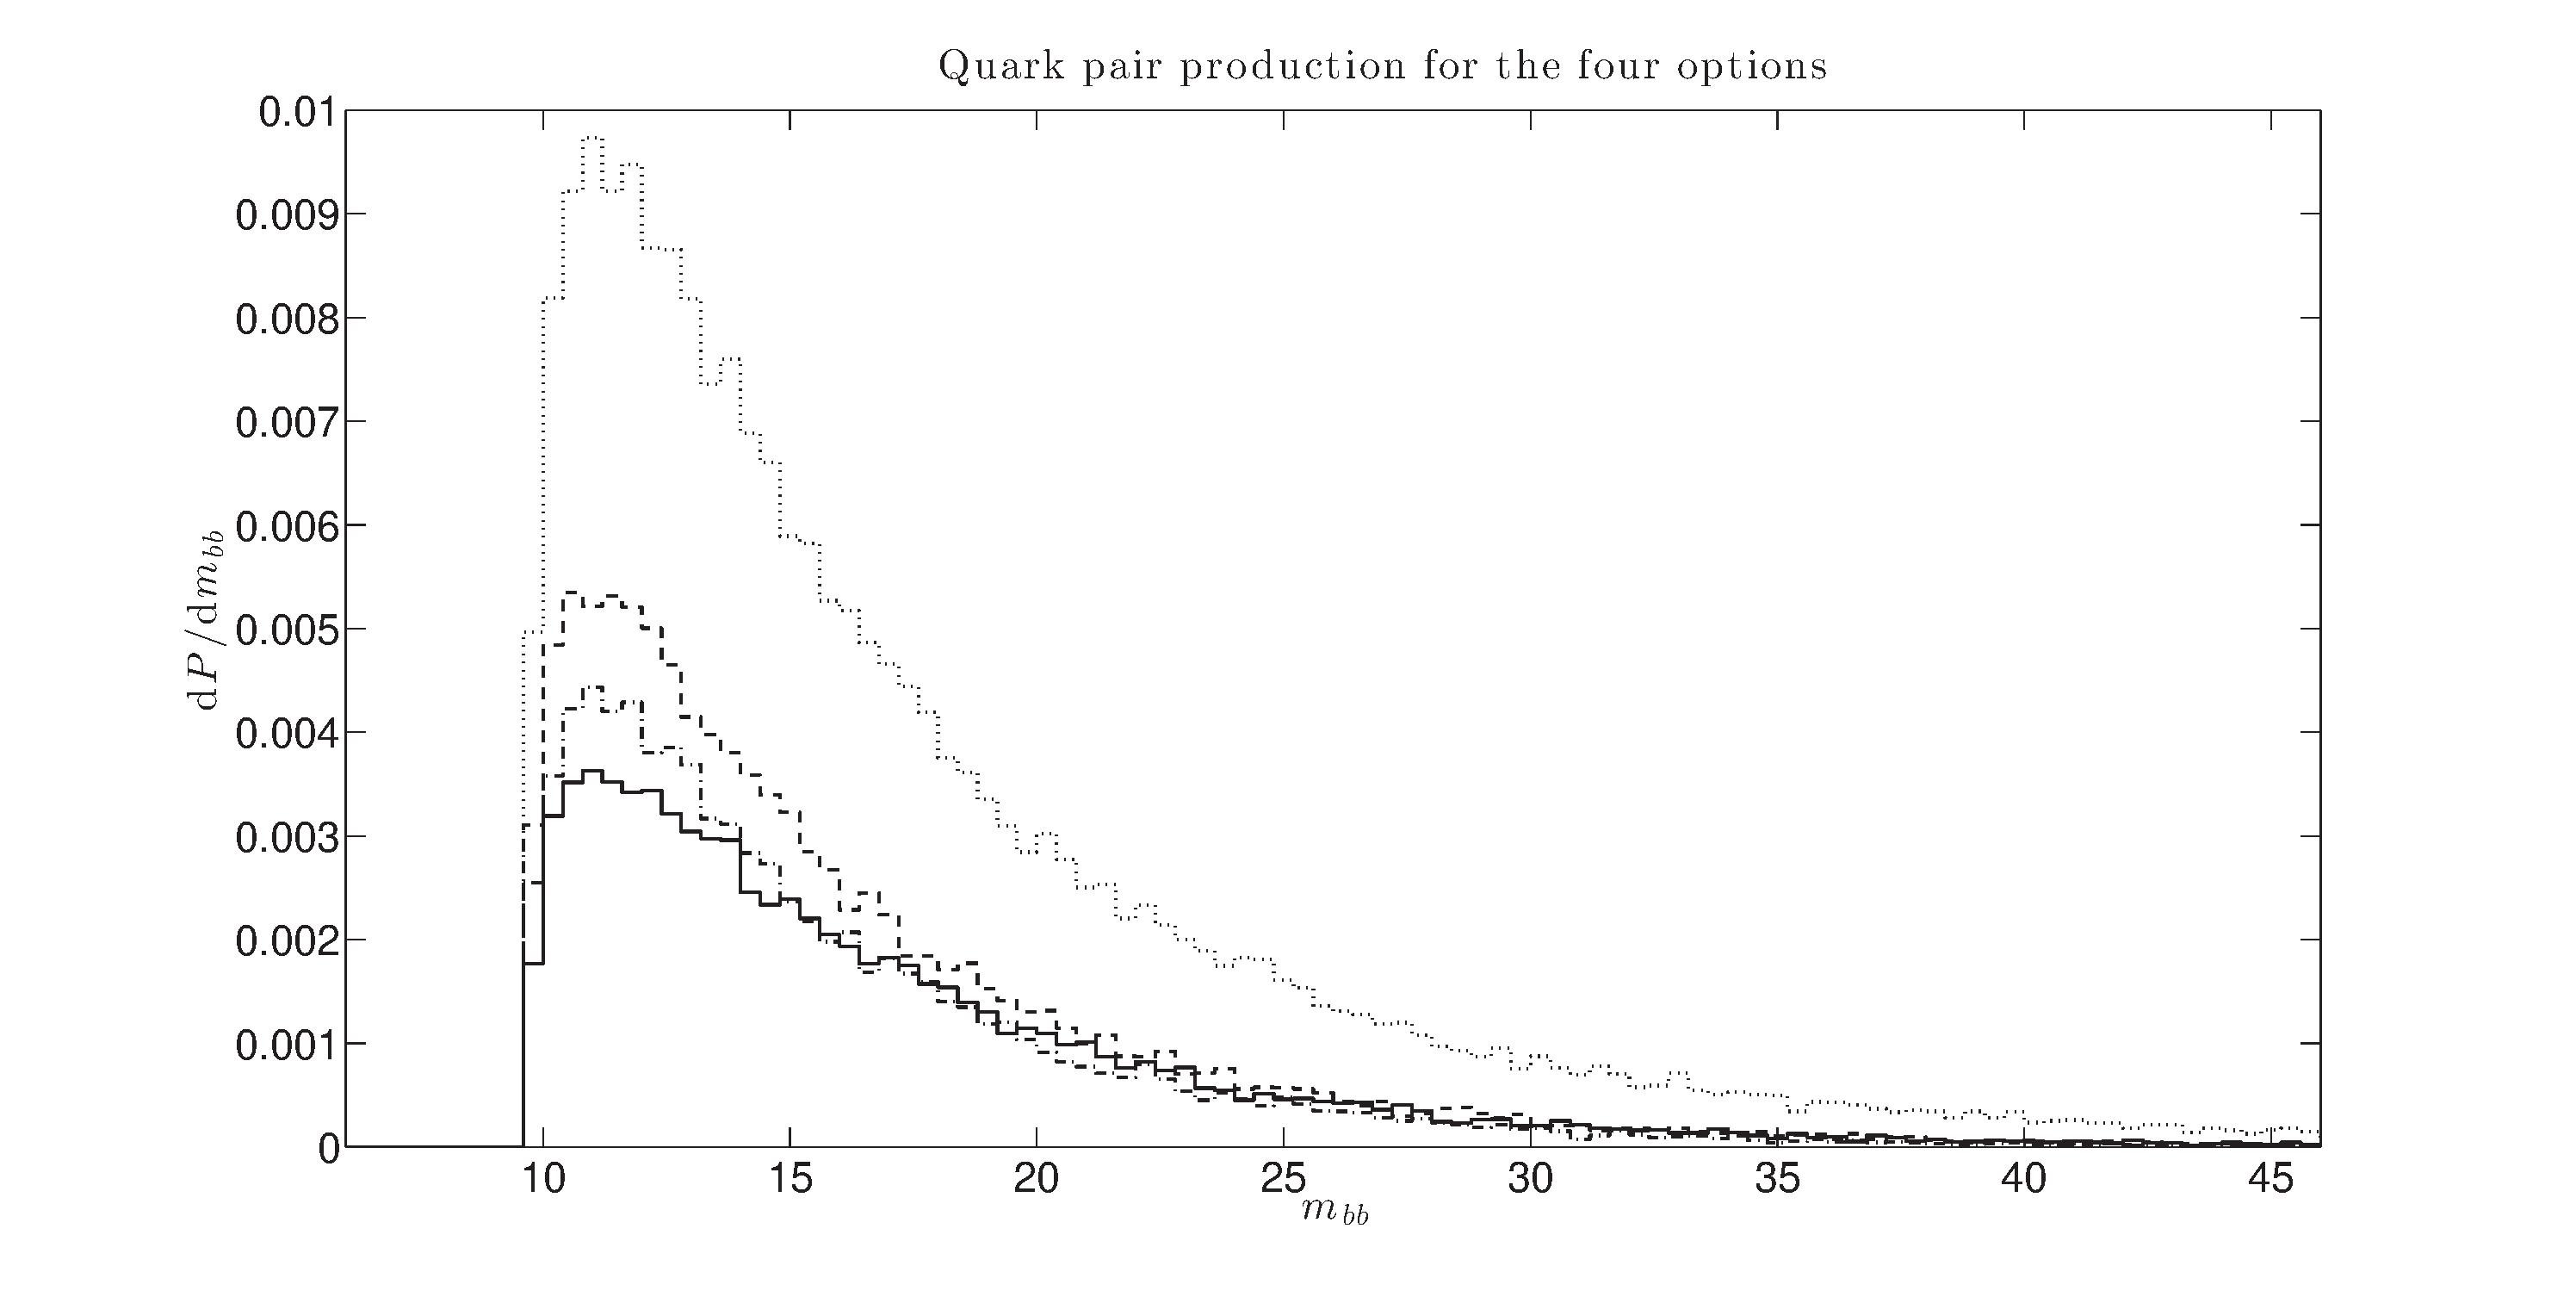
\includegraphics[width=15cm]{QMass.eps}
\label{fig:QMass}
\end{figure}
The relevant features of the options 1-4, discussed in \ref{subsubsec:PythiaAlg}, are present in this graph. Option 3 represents the extreme case. The compensation between the enhancement in the threshold region and the suppression for high masses in option 4 is visible. That compensation corrects the total rate (area under the curve) to a value similar to the one given by option 1. From first principles, there was no reason to expect these two effects to compensate as closely as they do in the total rate. Option 2 has a clear enhancement in the threshold region compared to option 1.

The rate for the options using $m^2$ as the evolution variable (5-8) have a slightly suppressed rate compared to the first four, around 5\% less.

The values given by options 1, 4, 5, 6 and 8 fit inside the total error of the last three references in table \ref{table:gbbMeasurements}. The value given by option 2 lies outside the errors, but still within two standard deviations. Options 3 and 7 do not seem to reproduce experimental data at all, since they show values well above the upper bound given by the error in all the measurements.

The discrepancies could be related to the mass of the bare $\b$ quark, a quantity that cannot be measured directly. Using a higher $m_\b$ than the default, the simulated rate would be reduced, matching better the experimental results. Furthermore, taking in account the systematic errors provided in table \ref{table:gbbMeasurements} and the spread in the values, we can notice that the measurement of this rate is a complicated one. 

\subsubsection{$\D^{*\pm}$ energy fraction spectrum}

We are going to study the production rate of $\D^{*\pm}$ mesons as a function of the energy fraction $X_E$. The ALEPH collaboration has provided measurements for this in \cite{Barate:1999bg}. The total spectrum is taken as the sum of three components: mesons coming from primary charms, from primary bottoms and from secondary heavy quarks, i.e., from gluon branchings.

\begin{figure}[h]
\centering
\caption[Energy fraction spectrum of the $\D^{*\pm}$ mesons.]{Energy fraction distribution for the $\D^{*\pm}$ mesons. The points with error bars are the measurements from ALEPH and the solid line is the \textsc{Pythia} simulation, with the respective contributions: $\b\bbar$ (dotted line), $\c\cbar$ (dashed line) and gluon branching (dashed-dotted).}
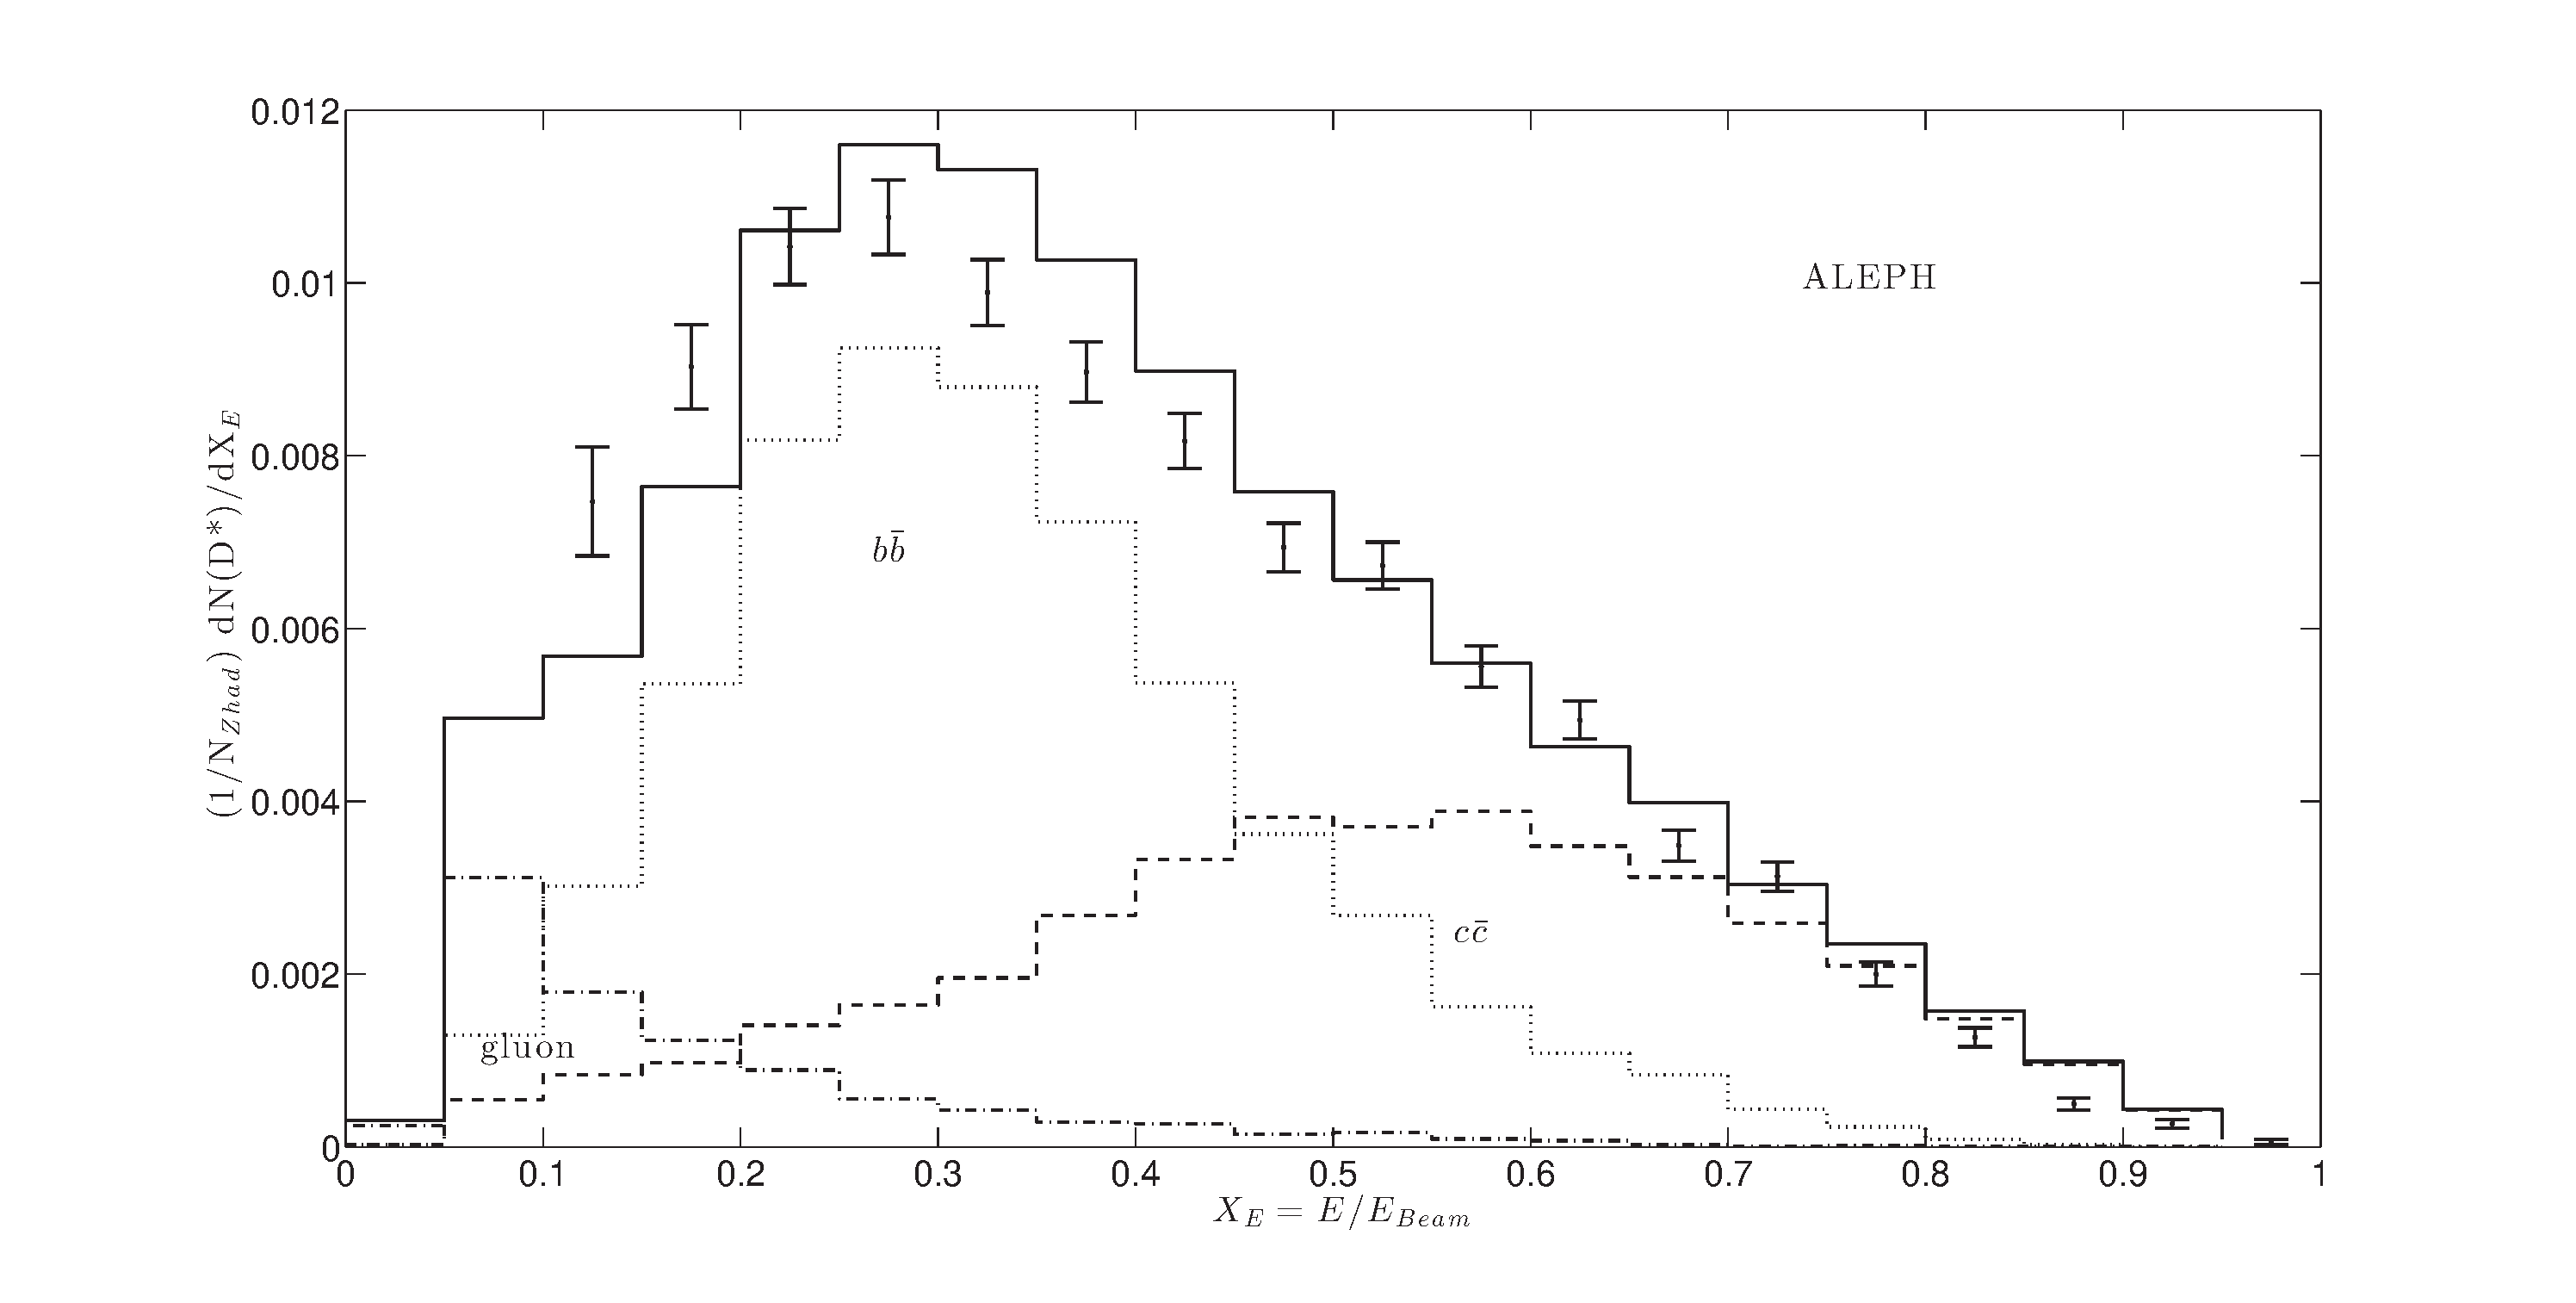
\includegraphics[width=15cm]{DStarOp1Thesis.eps}
\label{fig:ALEPHPythia1}
\end{figure}

The plot in fig. \ref{fig:ALEPHPythia1} shows the ALEPH measurements and the \textsc{Pythia} (option 1) simulation with the components. We can see that the main contribution of the gluon splitting is at low energy fractions, which is due to the fact that the secondary quarks are produced at least at a third branching from the $Z^0$ (as in fig. \ref{fig:PrimSecQuarks}), where the energy has been distributed into several products. Then, the main impact of the options will be at low energy fractions. The figure also suggests the need for a correction at low energy fractions, in addition to the primary $\c\cbar$ and $\b\bbar$ components. Also, the simulation presents an excess just after the peak near 0.3. For high $X_E$ simulation and measurements are in good agreement.

Figure \ref{fig:GluonDStar} shows the extreme cases for the gluon contribution: options 1 and 3. The latter gives values at least two times higher that the former in each bin. The distributions for the options 2 and 4 (not shown) give intermediate values.

\begin{figure}[h]
\centering
\caption[Gluon contribution to the $\D^{*\pm}$ production in two extreme cases.]{Extreme cases of the $\D^*$ production from gluons. \textsc{Pythia} options 1 (solid) and 3 (dashed).}
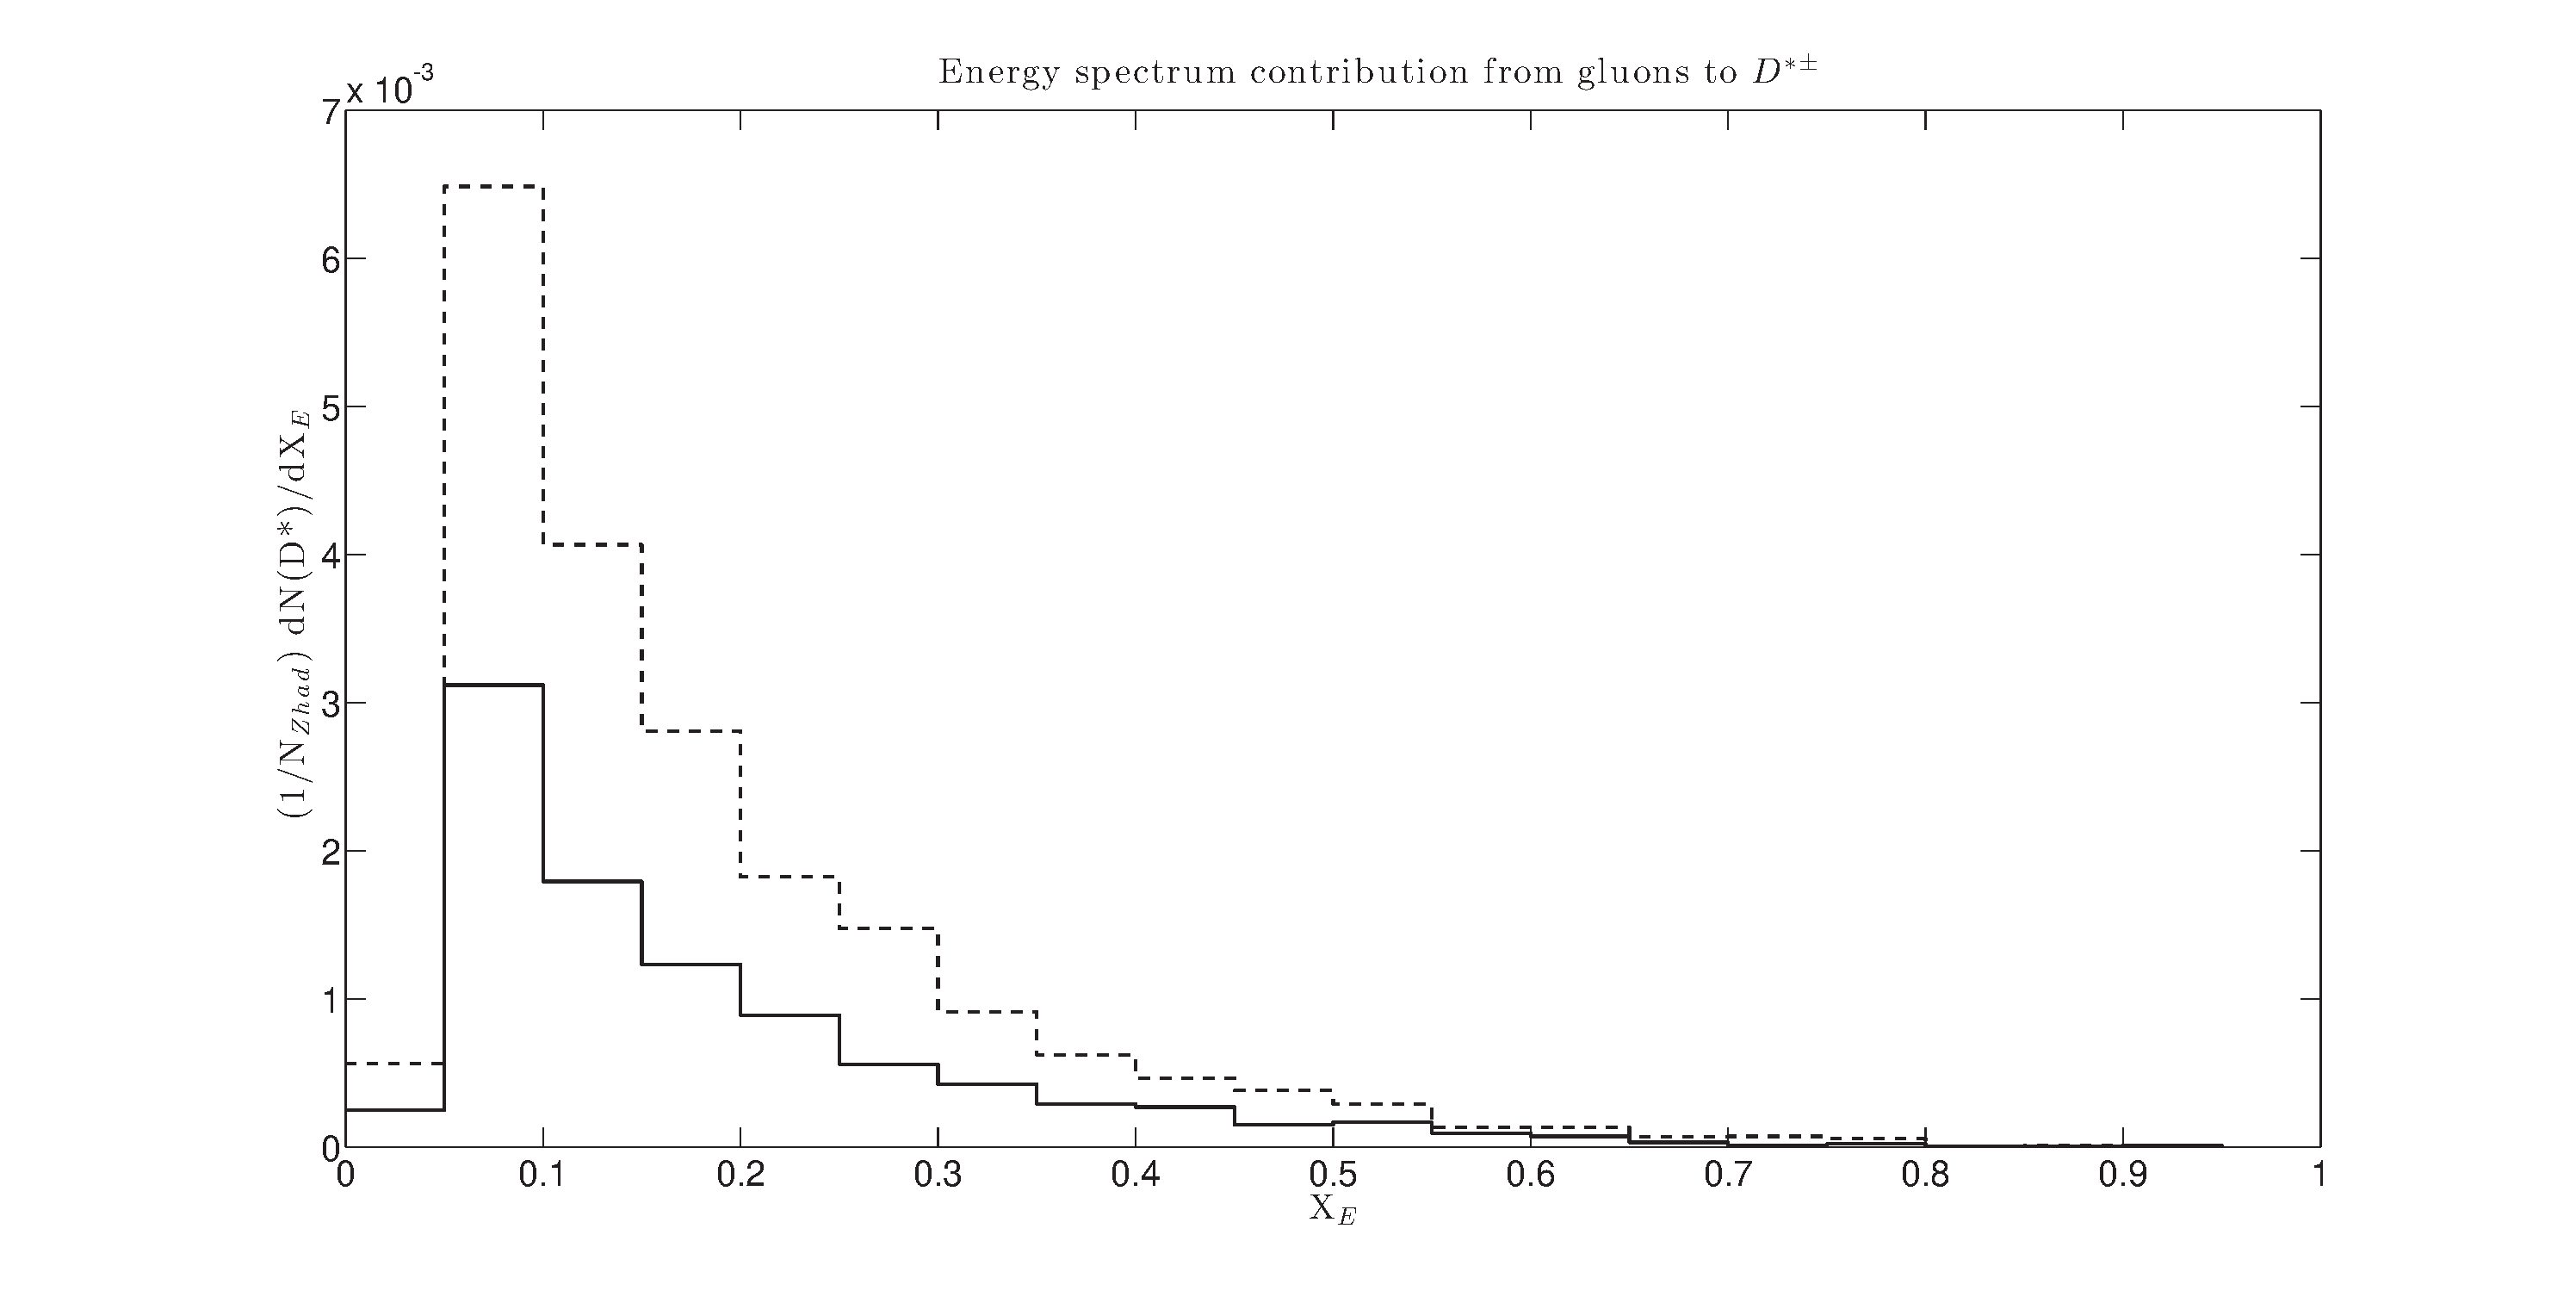
\includegraphics[width=15cm]{GluonDStarThesis.eps}
\label{fig:GluonDStar}
\end{figure}

To compare the four options with the experimental data, figure \ref{fig:DStarOp} shows the full distributions and the ALEPH measurements. The enhancement at low energies is evident for the non-default options, where the simulations get closer to the experimental values. The excess near the peak is still present and slightly enhanced. At high energies, the decreasing tails show no major differences (since the main contribution is due to the primary production in this region) and follow approximately the behaviour of the data.

\begin{figure}[!h]
\centering
\caption[$\D^{*\pm}$ energy fraction spectrum. Simulations and data compared.]{$\D^{*\pm}$ energy fraction spectrum. ALEPH data (dots with error bars) and \textsc{Pythia} options: default (solid), 2 (dotted), 3 (dashed) and 4 (dashed-dotted).}
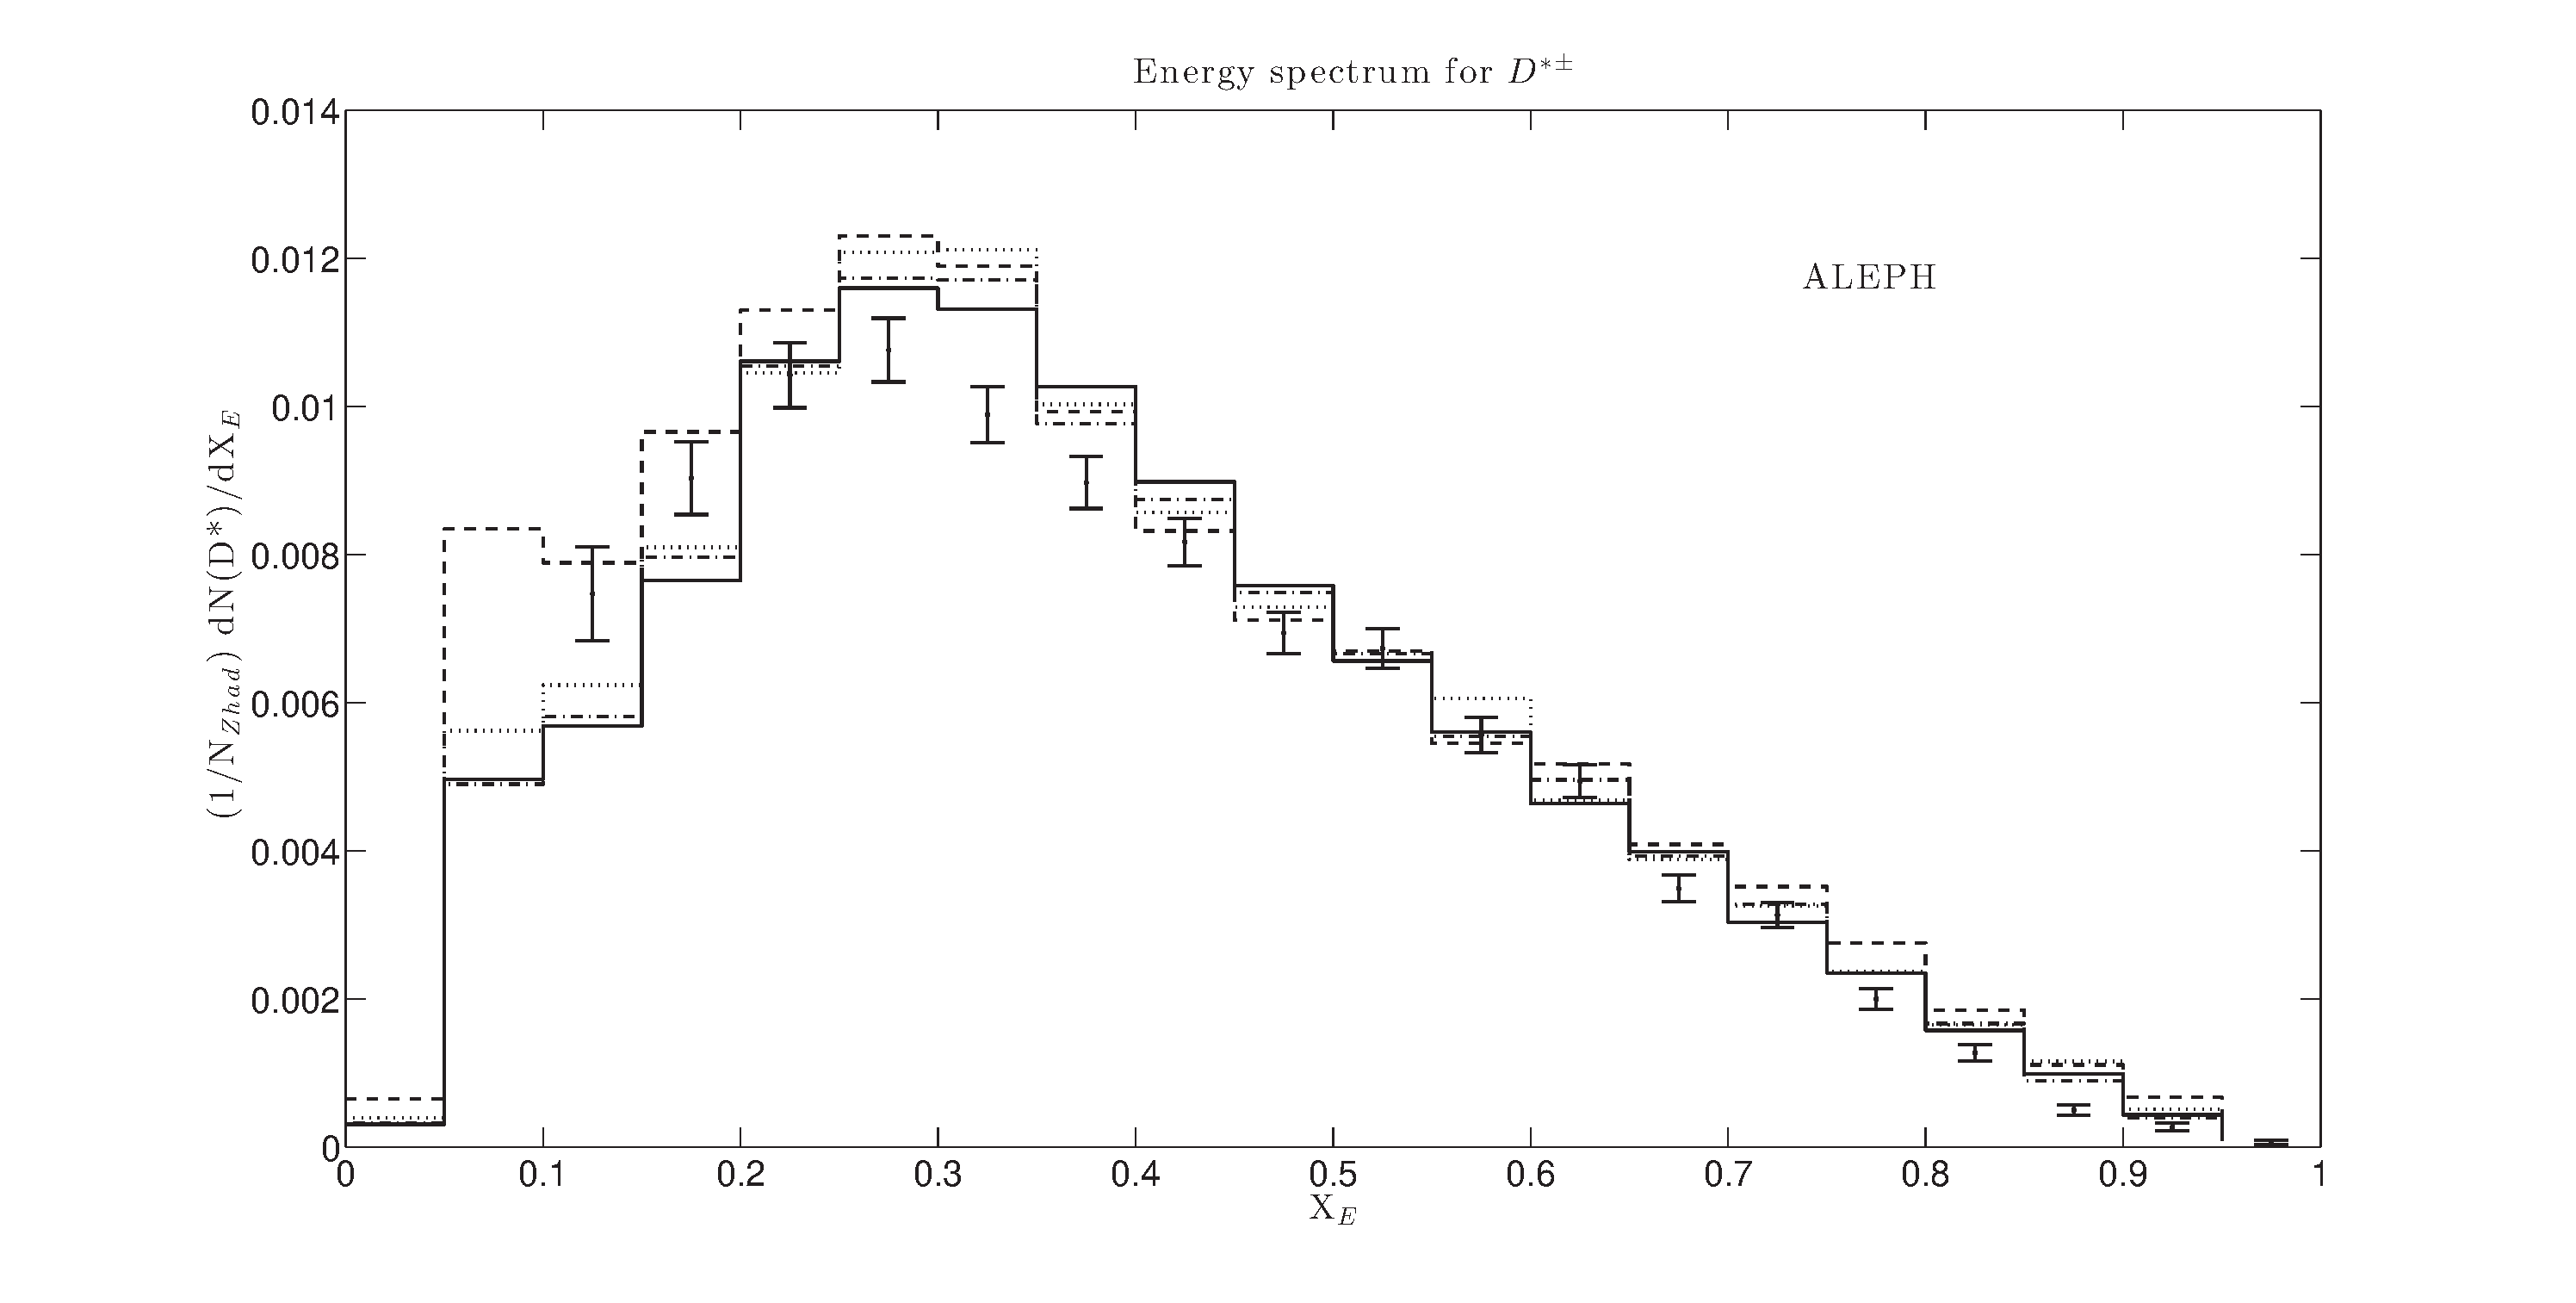
\includegraphics[width=15cm]{DStarOpThesis.eps}
\label{fig:DStarOp}
\end{figure}

In this context, option 3 seems a good candidate, since it corrects (somehow accurately) the $\D^*$ production at low energy fractions. For the region just after the peak, the enhancement might be higher than desired, but still the data is closer to this option, overall.

Due to their non-perturbative character, meson decays are not fully understood. A slightly different modelling of the $\B\to\D$ decay could shift some events above the peak to below it, better fitting the data in both regions, without requiring a higher $\g\to\b\bbar$ rate. The study is therefore inconclusive regarding this issue. 

\subsection{Proton-proton collisions at 7000 GeV}

Turning now to hadron collisions, we will study the correlations between $\B$ hadron pairs. Events with one pair are classified as PC, FE or GS; events with more pairs are classified as mixed.

A $5\times 10^6$ events simulation was done for each option. Events with two $\B$ mesons, each of them with a trasverse momentum greater than 15 GeV, are selected to the analysis. A lowest transverse momentum cutoff for the hard process of 15 GeV is also imposed. This is necessary since the events with lower $\pT$ are more likely to be produced, but the number of selected events decrease for values lower than 20 GeV, as one can see in fig. \ref{fig:accepted}. There, only around 1\% of the events are selected to the analysis. An even lower cutoff would increase such ``inefficiency'', with only few more selected events in comparison to the total number of generated ones.

\begin{figure}[h]
\centering
\caption[Generated and accepted events in hadron collisions.]{Generated (solid) and accepted (dashed) events as a a function of the transverse momentum of the hard process.}
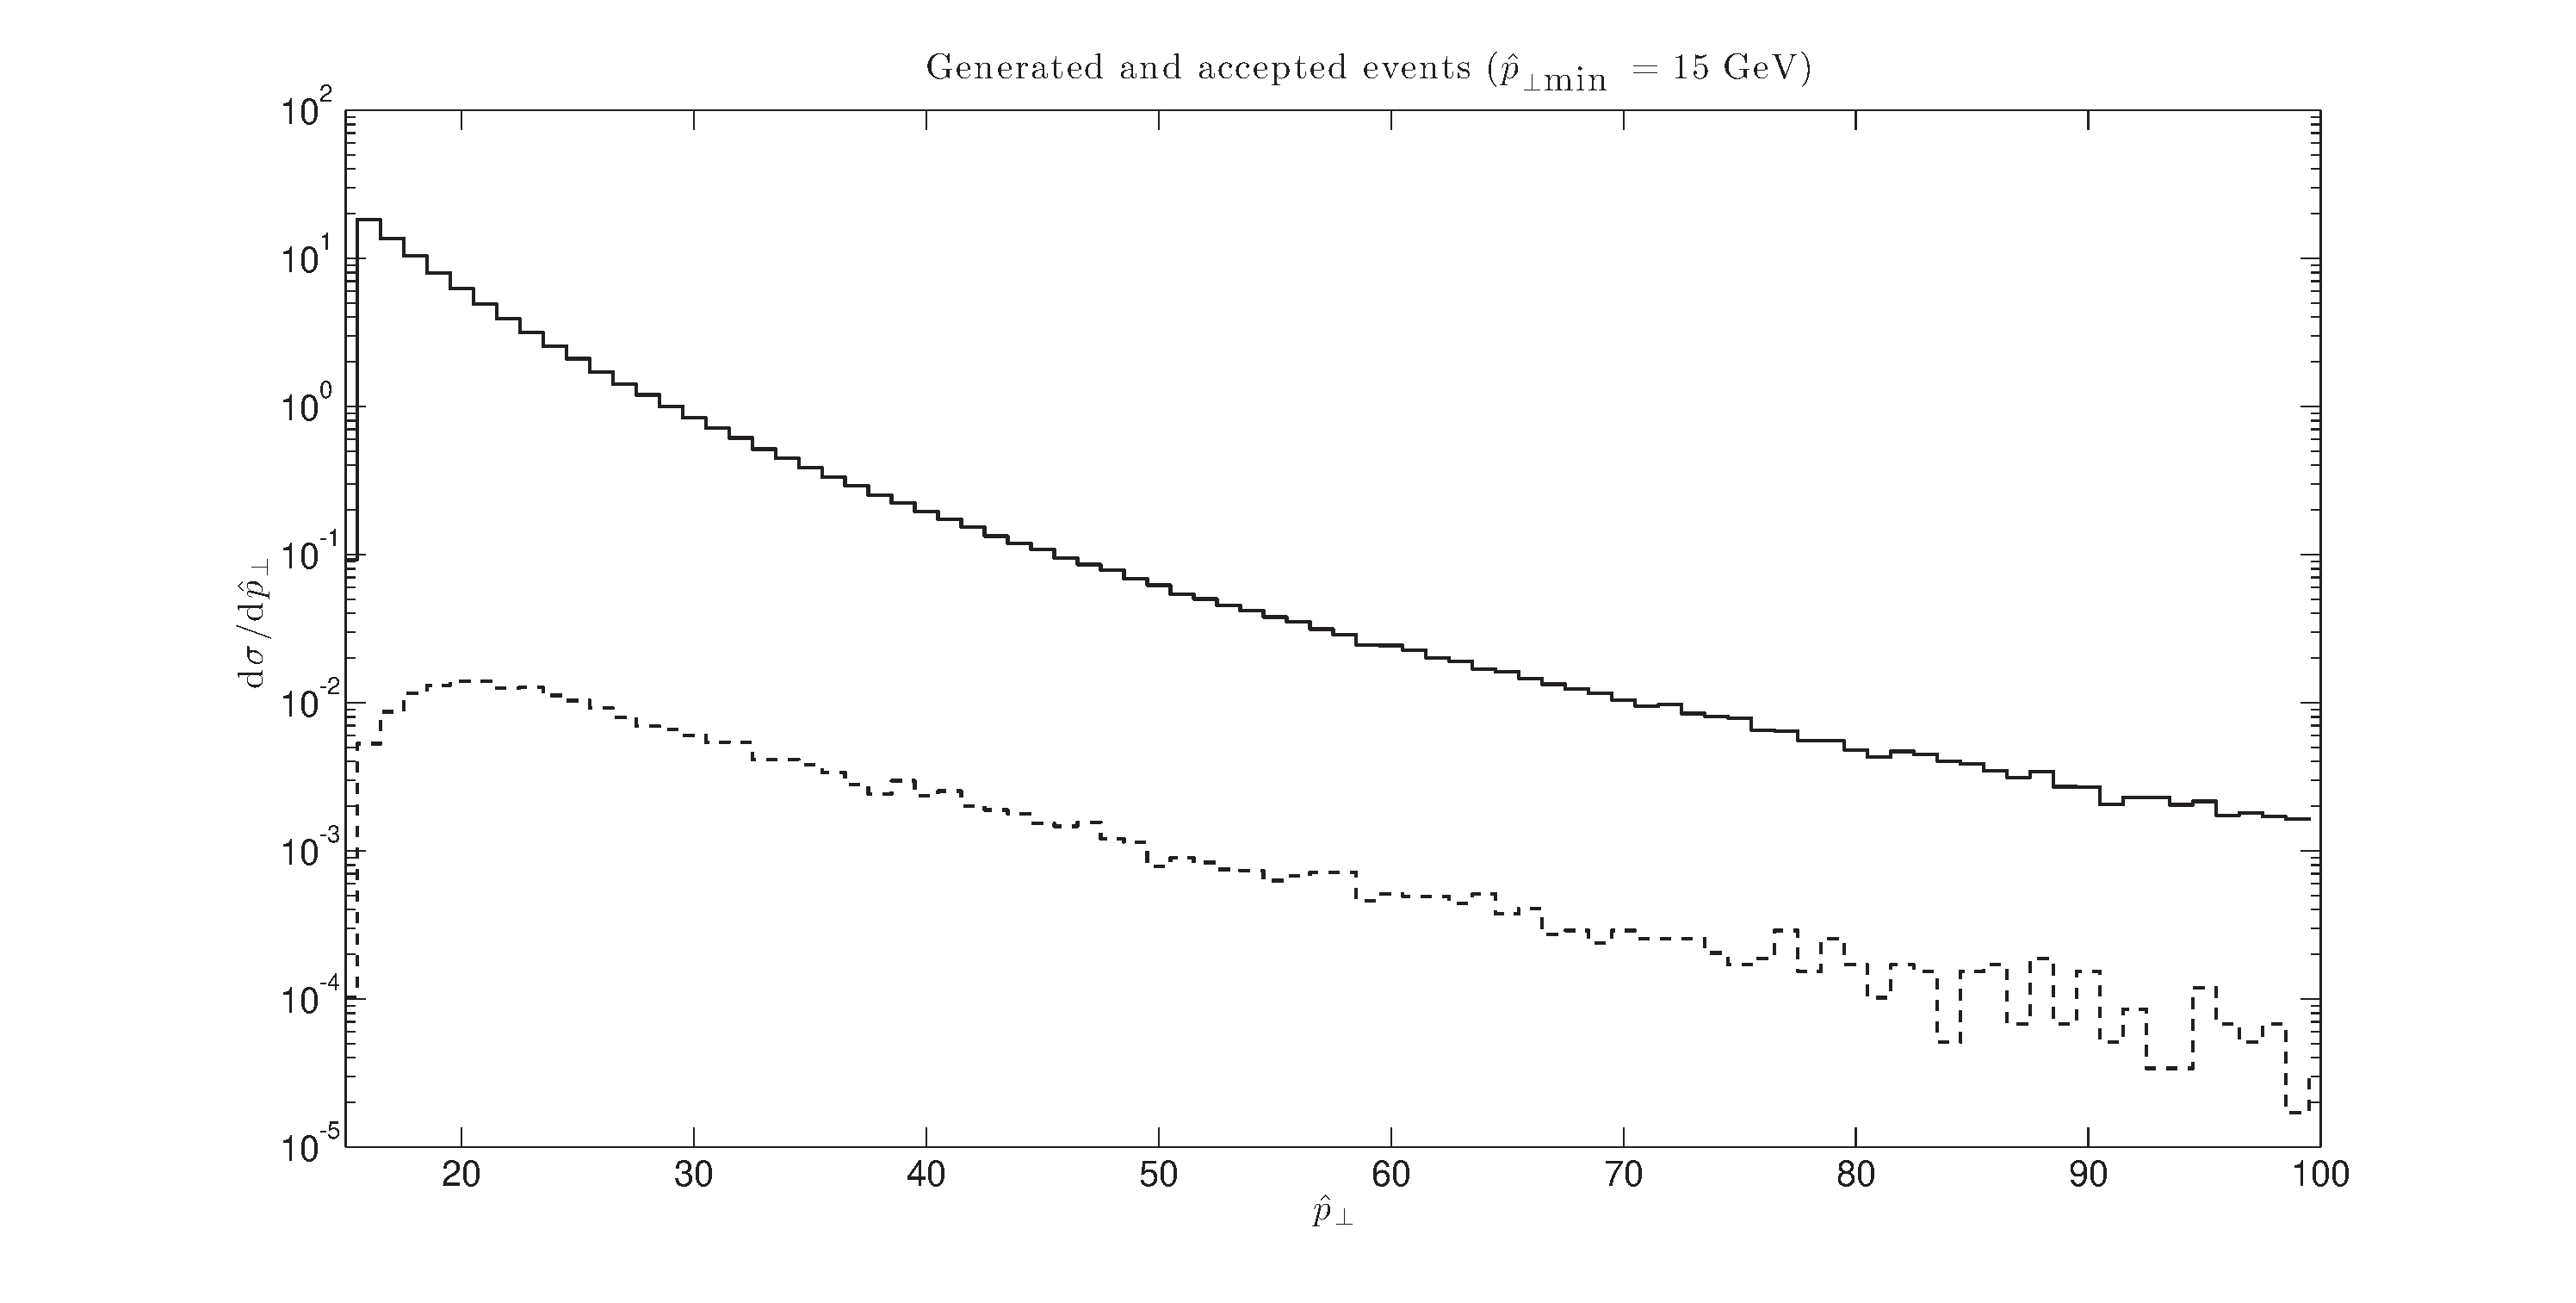
\includegraphics[width=15cm]{Accepted.eps}
\label{fig:accepted}
\end{figure}

\subsubsection{Azimuthal angular separations}

The variation of the azimuthal angle is a good measure of the separation of two $\B$ mesons, since it is invariant under Lorentz boosts along the beam axis ($z$). The difference $\Delta \varphi$ is measured in the plane perpendicular to the $z$-axis. Figure \ref{fig:BBPhiOp1} shows the production of bottom meson pairs in terms of the azimuthal angular separation, for option 1.

\begin{figure}[!h]
\centering
\caption[$\B$ meson pairs azimuthal angular separation. \textsc{Pythia} default option.]{Azimuthal angular separation of $\B$ mesons pairs using \textsc{Pythia} default option, including the four sources.}
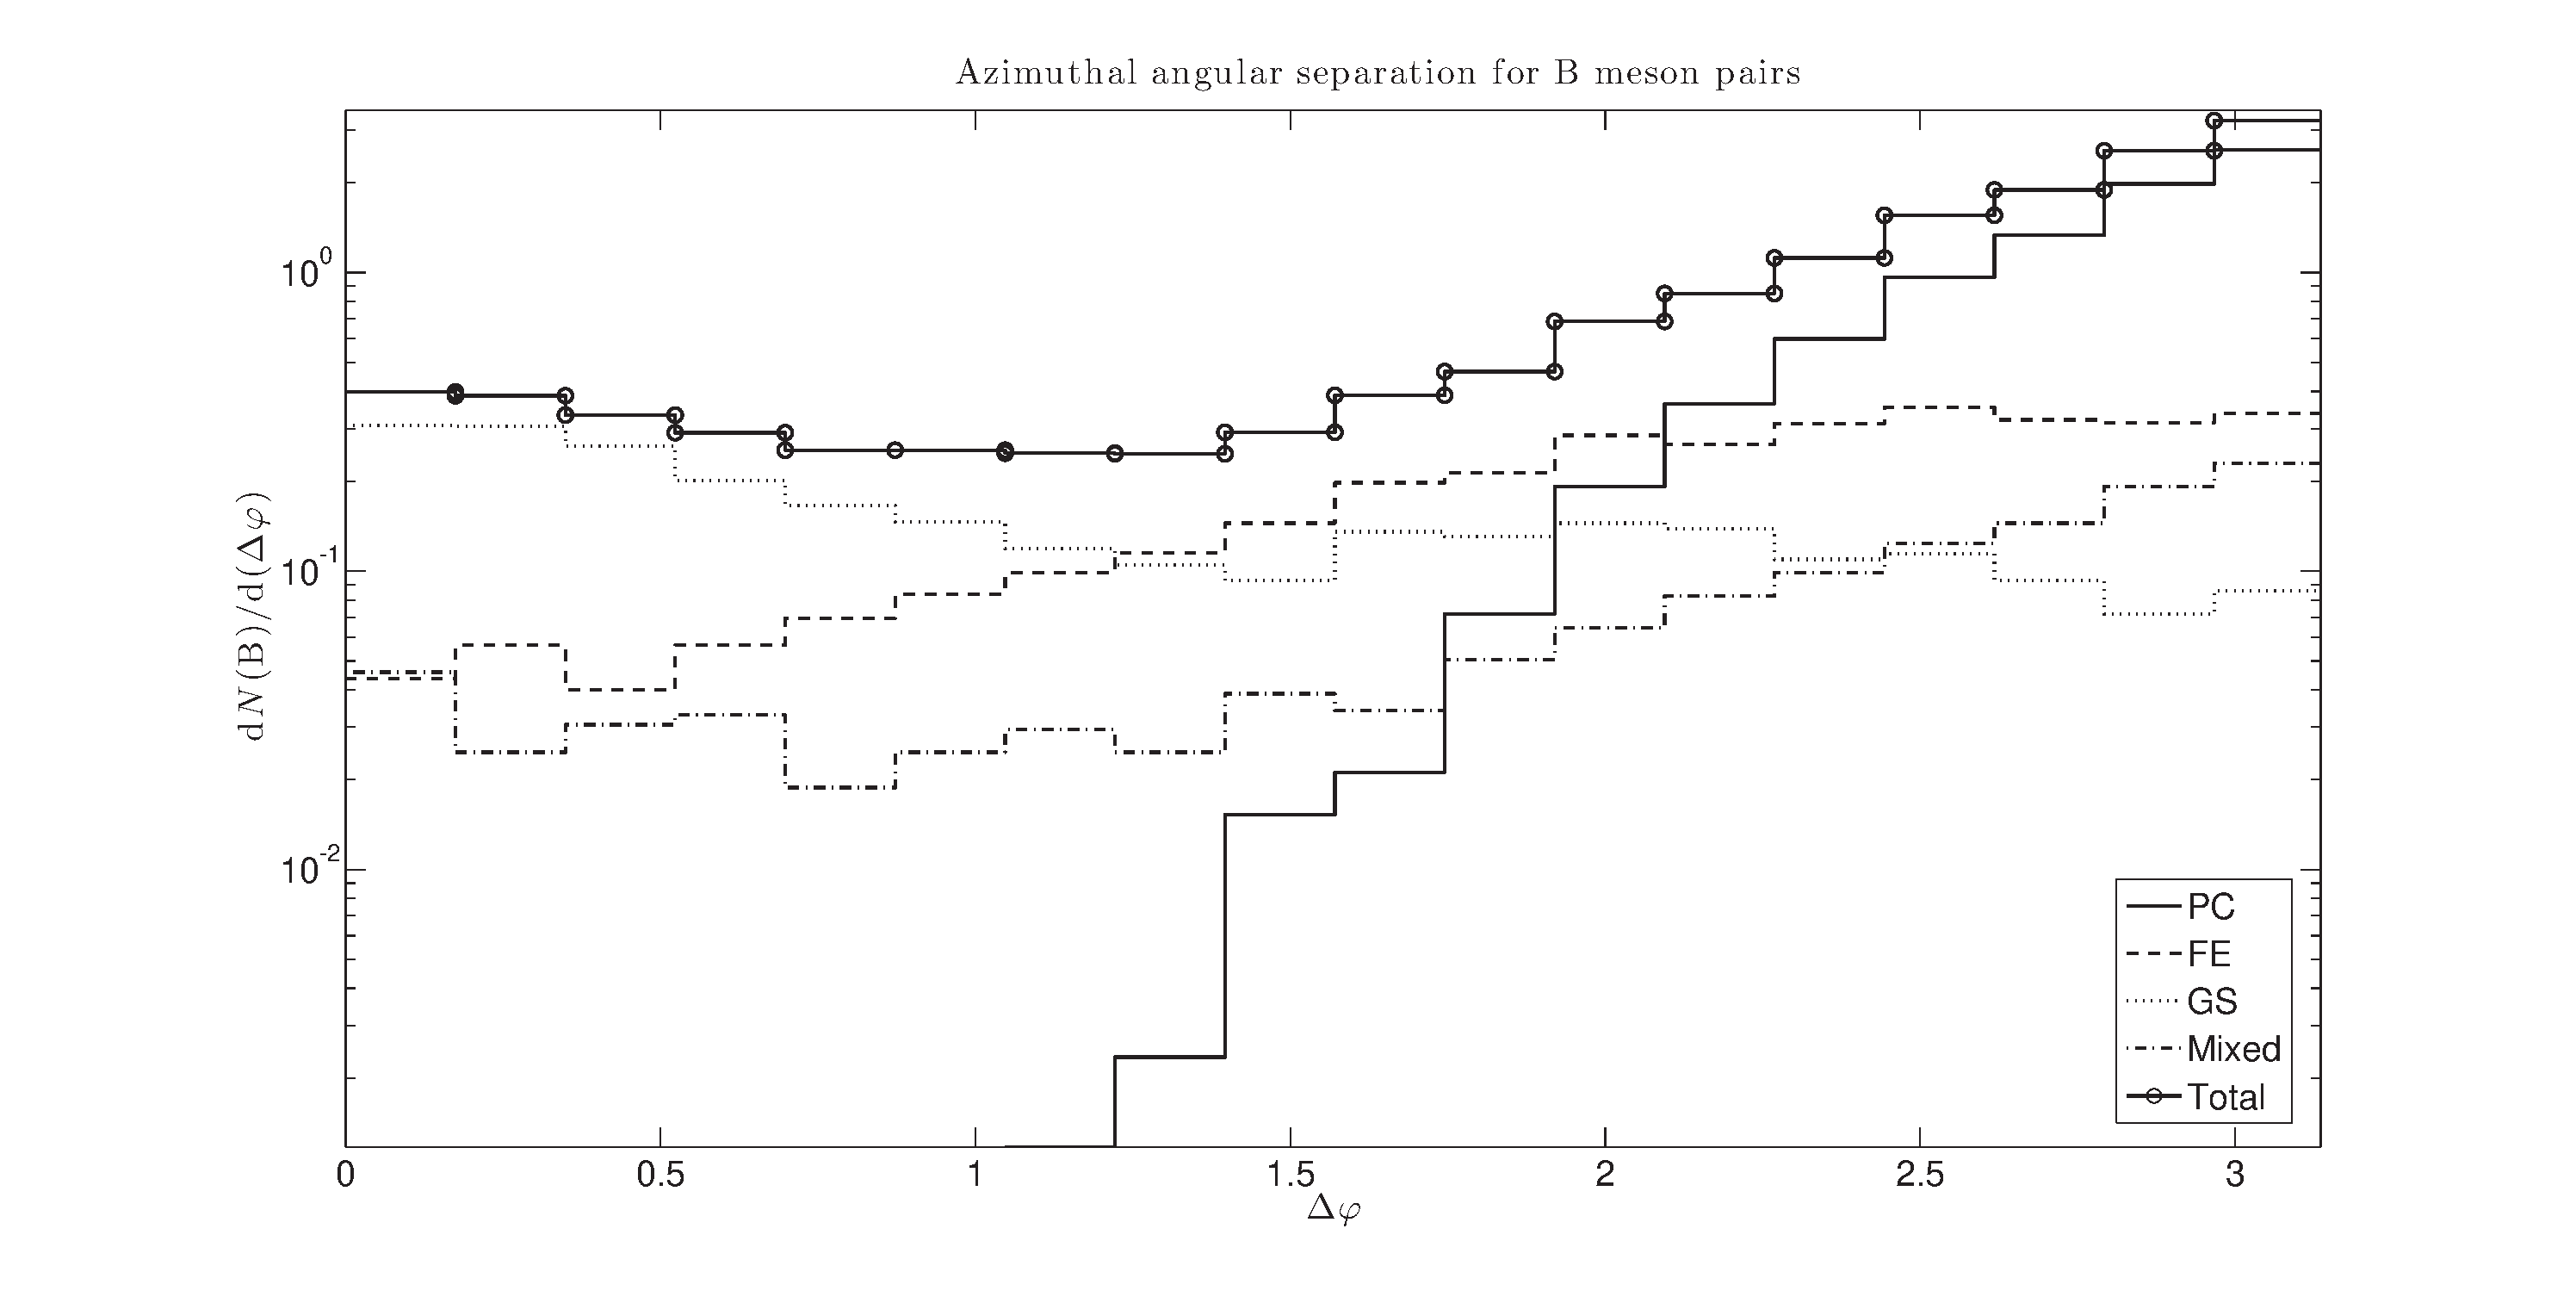
\includegraphics[width=15cm]{BBPhiOp1.eps}
\label{fig:BBPhiOp1}
\end{figure}
First features of the correlations in the production mechanisms are revealed: PC peaks at high angles, since the pairs created in the hard process tend to be back-to-back, whereas GS contributes mostly to the low-opening region. Pairs created by means of FE are less anticorrelated than the ones from PC. Mixed B mesons show an expected homogeneous angular distribution, because there is no particular relation between mesons coming from different gluon branchings.

The variation of the \textsc{Pythia} options is shown in fig. \ref{fig:BBPhi4Op}.

\begin{figure}[!h]
\centering
\caption[$\B$ meson pairs azimuthal angular separation. Four \textsc{Pythia} options.]{Azimuthal angular separation of $\B$ mesons pairs using \textsc{Pythia} options 1 (solid), 2 (dashed), 3 (dotted) and 4 (dashed-dotted).}
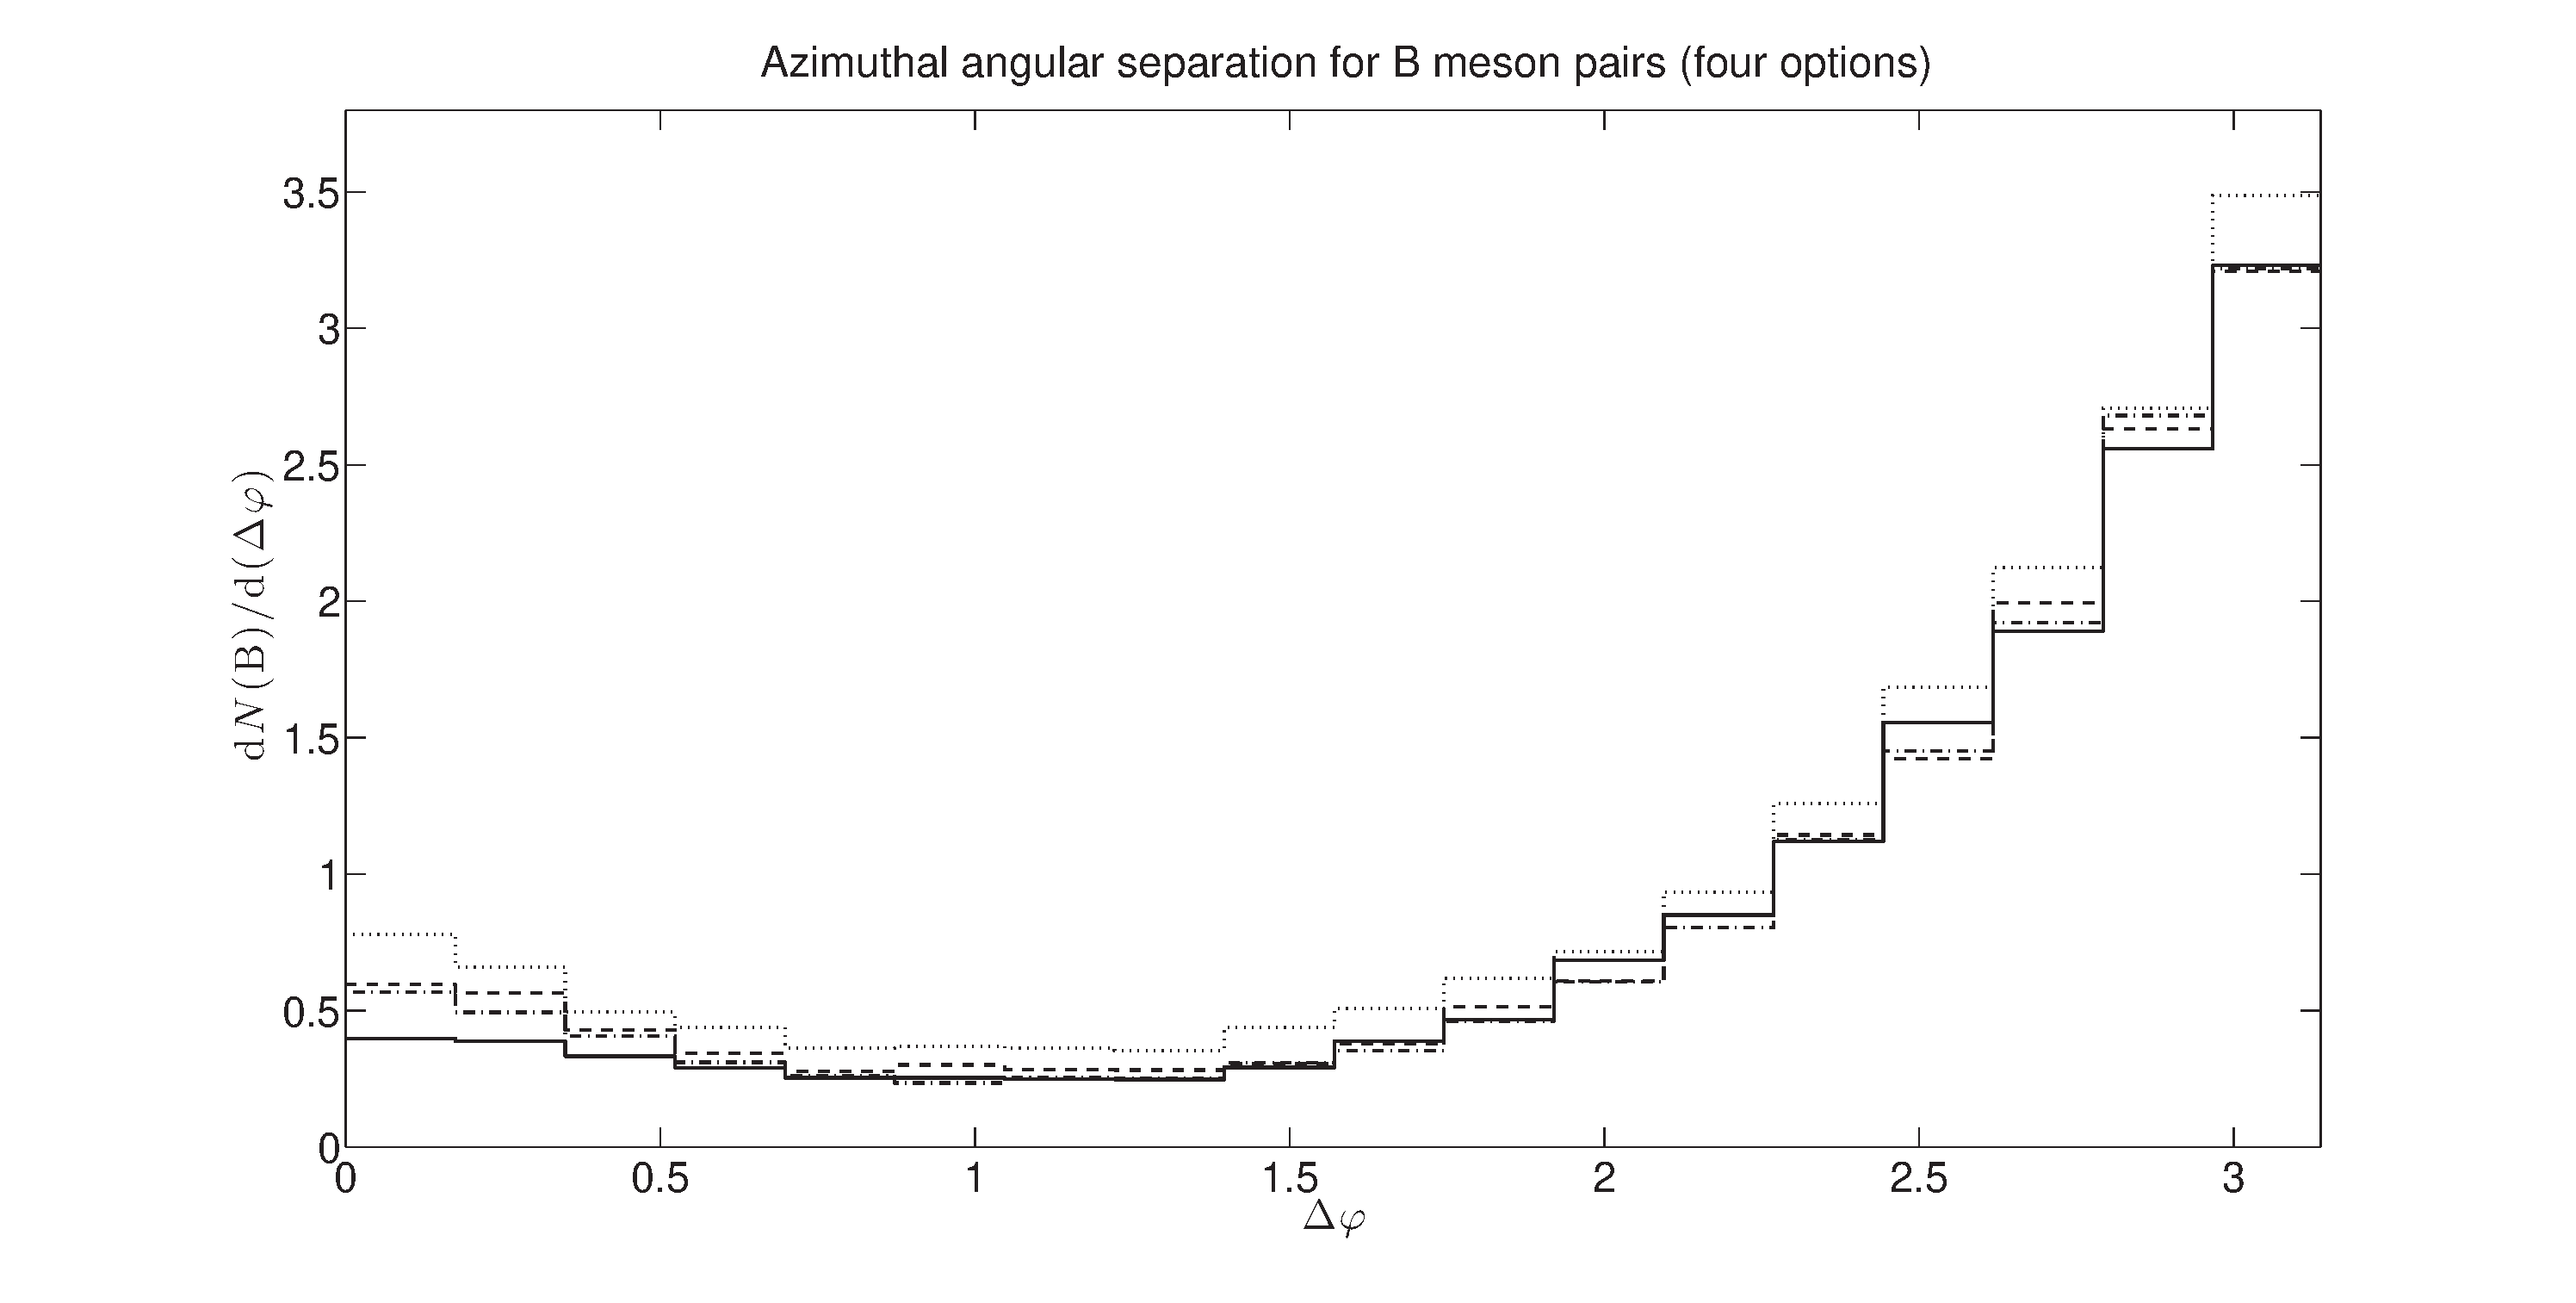
\includegraphics[width=15cm]{BBPhi4Op.eps}
\label{fig:BBPhi4Op}
\end{figure}
Similar to the case discussed in the previous subsection, the two upper and lower extreme cases at low azimuthal angles are given by options 3 and 1, where the gluon splitting dominates. Option 2 and 4 are intermediate in that region.

\subsubsection{Relative rapidities}

Rapidity, defined as
$$
y =\frac12 \ln \frac{E+p_z}{E-p_z},
$$
is a measure of the separation of the particle to the $z$ axis. In fact, it is related to the polar angle (between the particle and the $z$ axis). It can be shown that the difference $\Delta y \equiv y_2 - y_1$ is invariant under a $z$-axis boost.

The plot in figure \ref{fig:BBYOp1} shows the production of B meson pairs as a function of the relative rapidities $\Delta y$, as simulated with the default \textsc{Pythia} option.

\begin{figure}[!h]
\centering
\caption[$\B$ meson pairs relative rapidity. \textsc{Pythia} default option.]{Relative rapidity of $\B$ meson pairs using \textsc{Pythia} default option, including the four sources.}
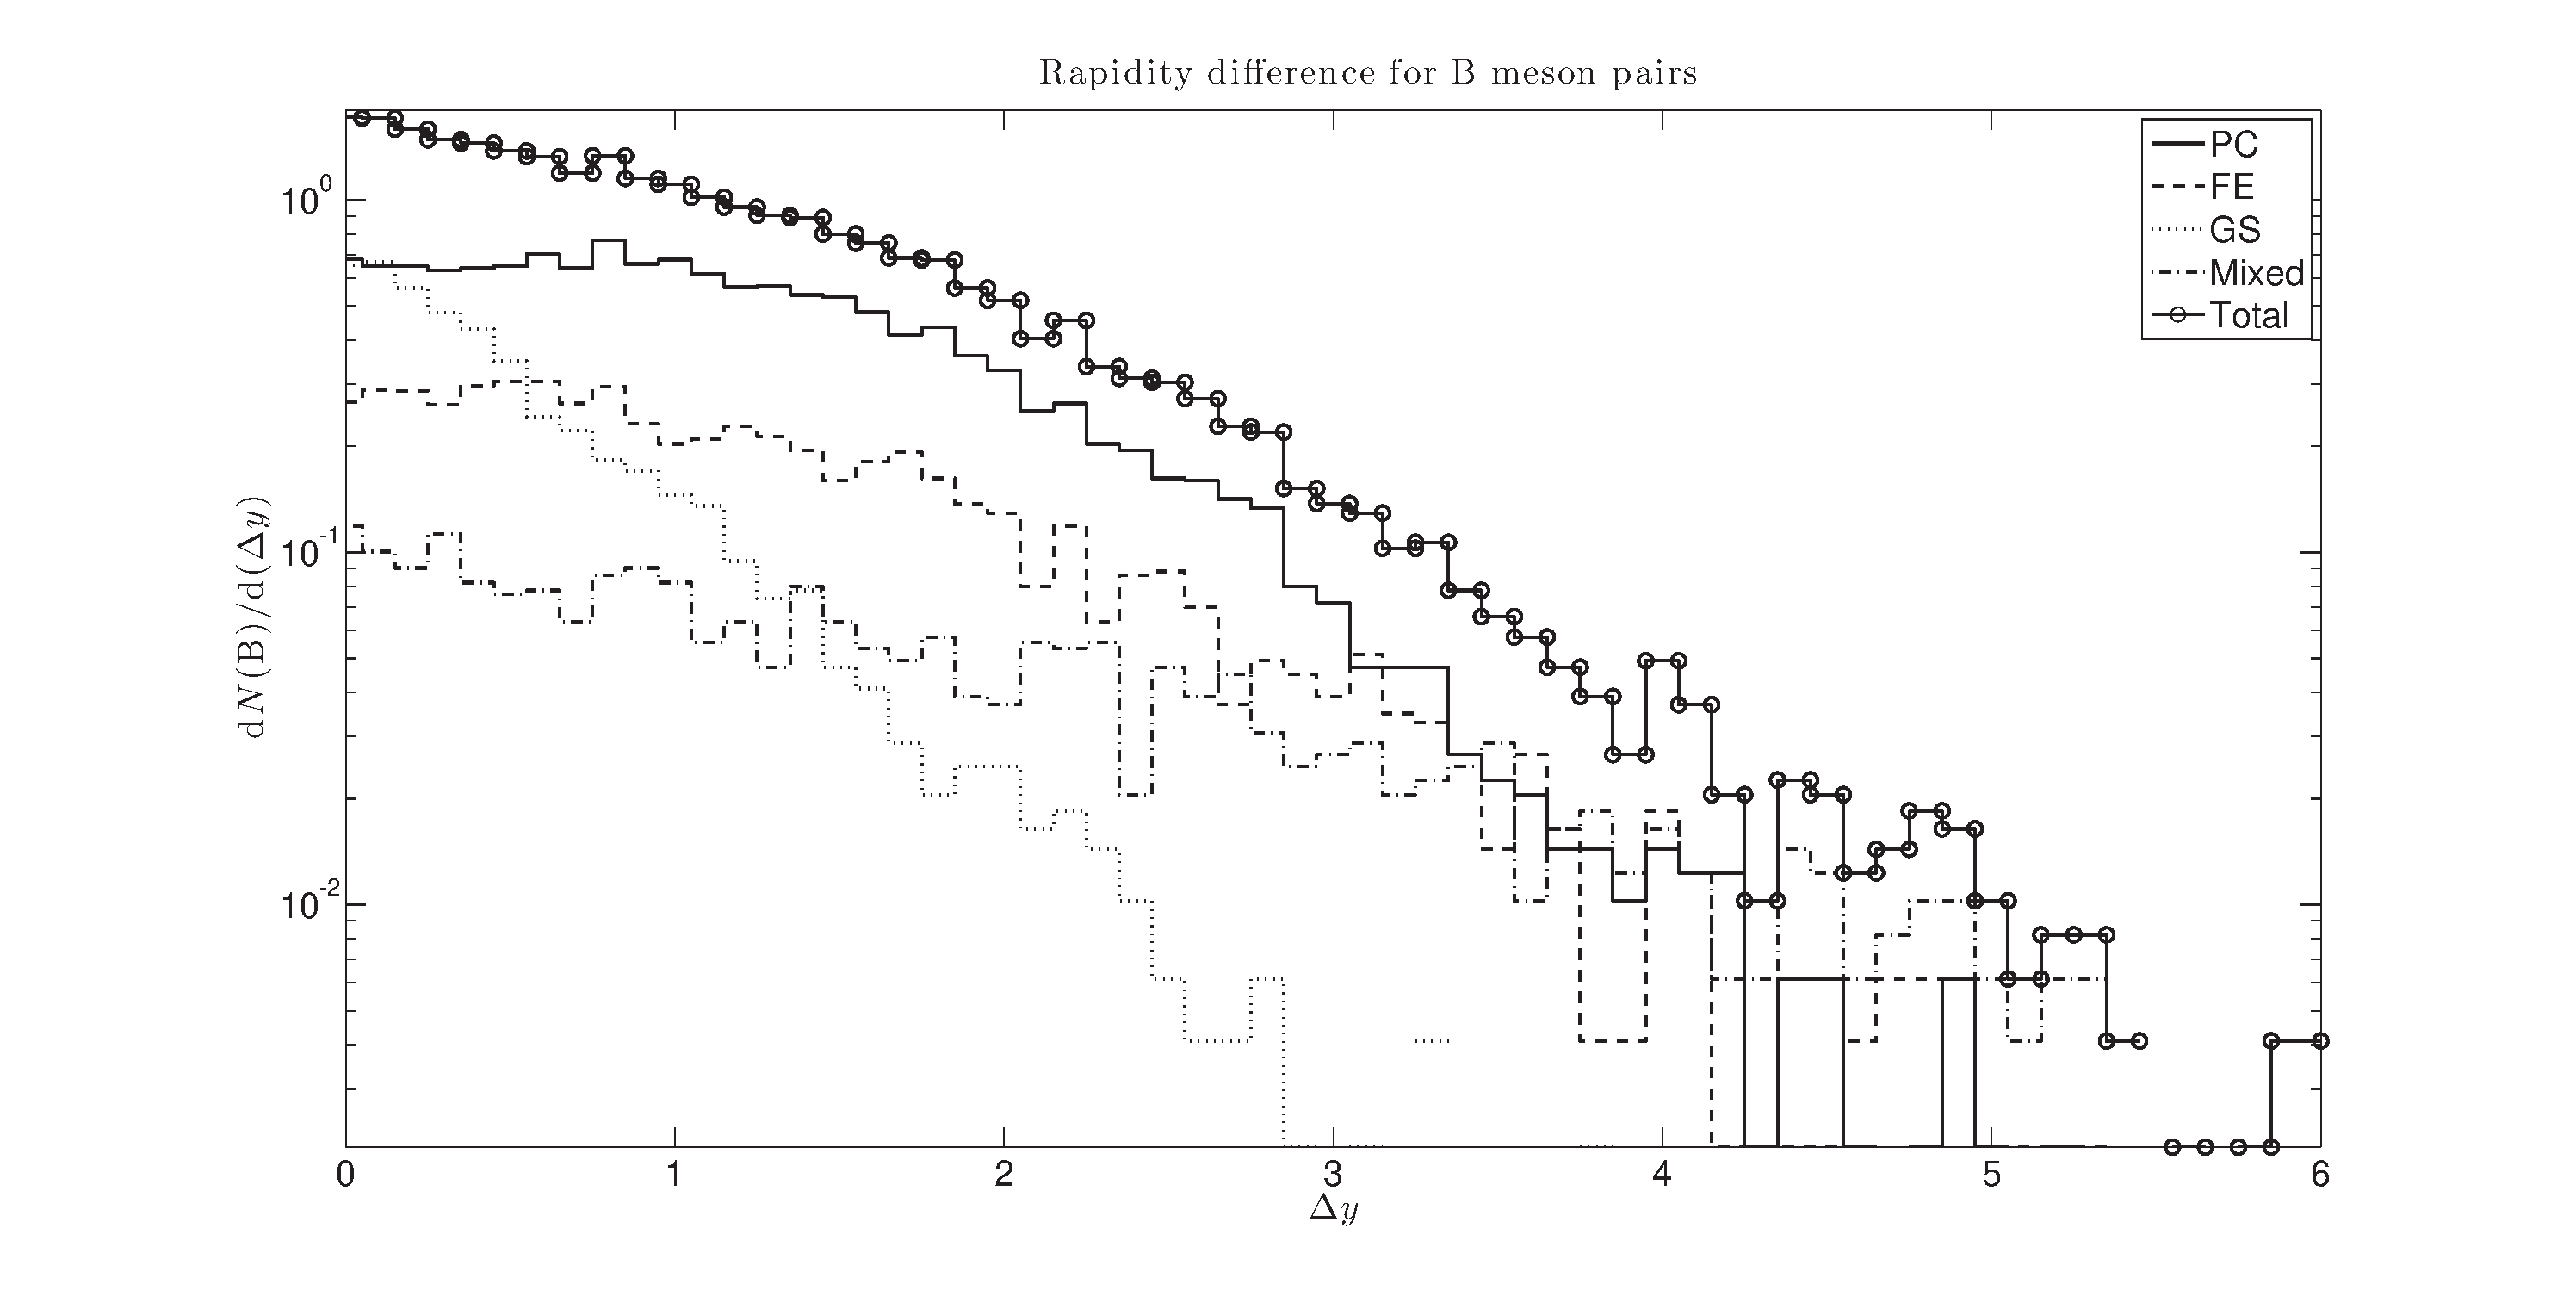
\includegraphics[width=15cm]{BBYOp1.eps}
\label{fig:BBYOp1}
\end{figure}

\begin{figure}[!h]
\centering
\caption[$\B$ meson pairs relative rapidity. Four \textsc{Pythia} options.]{Relative rapidity of $\B$ meson pairs using \textsc{Pythia} options 1 (solid), 2 (dashed), 3 (dotted) and 4 (dashed-dotted).}
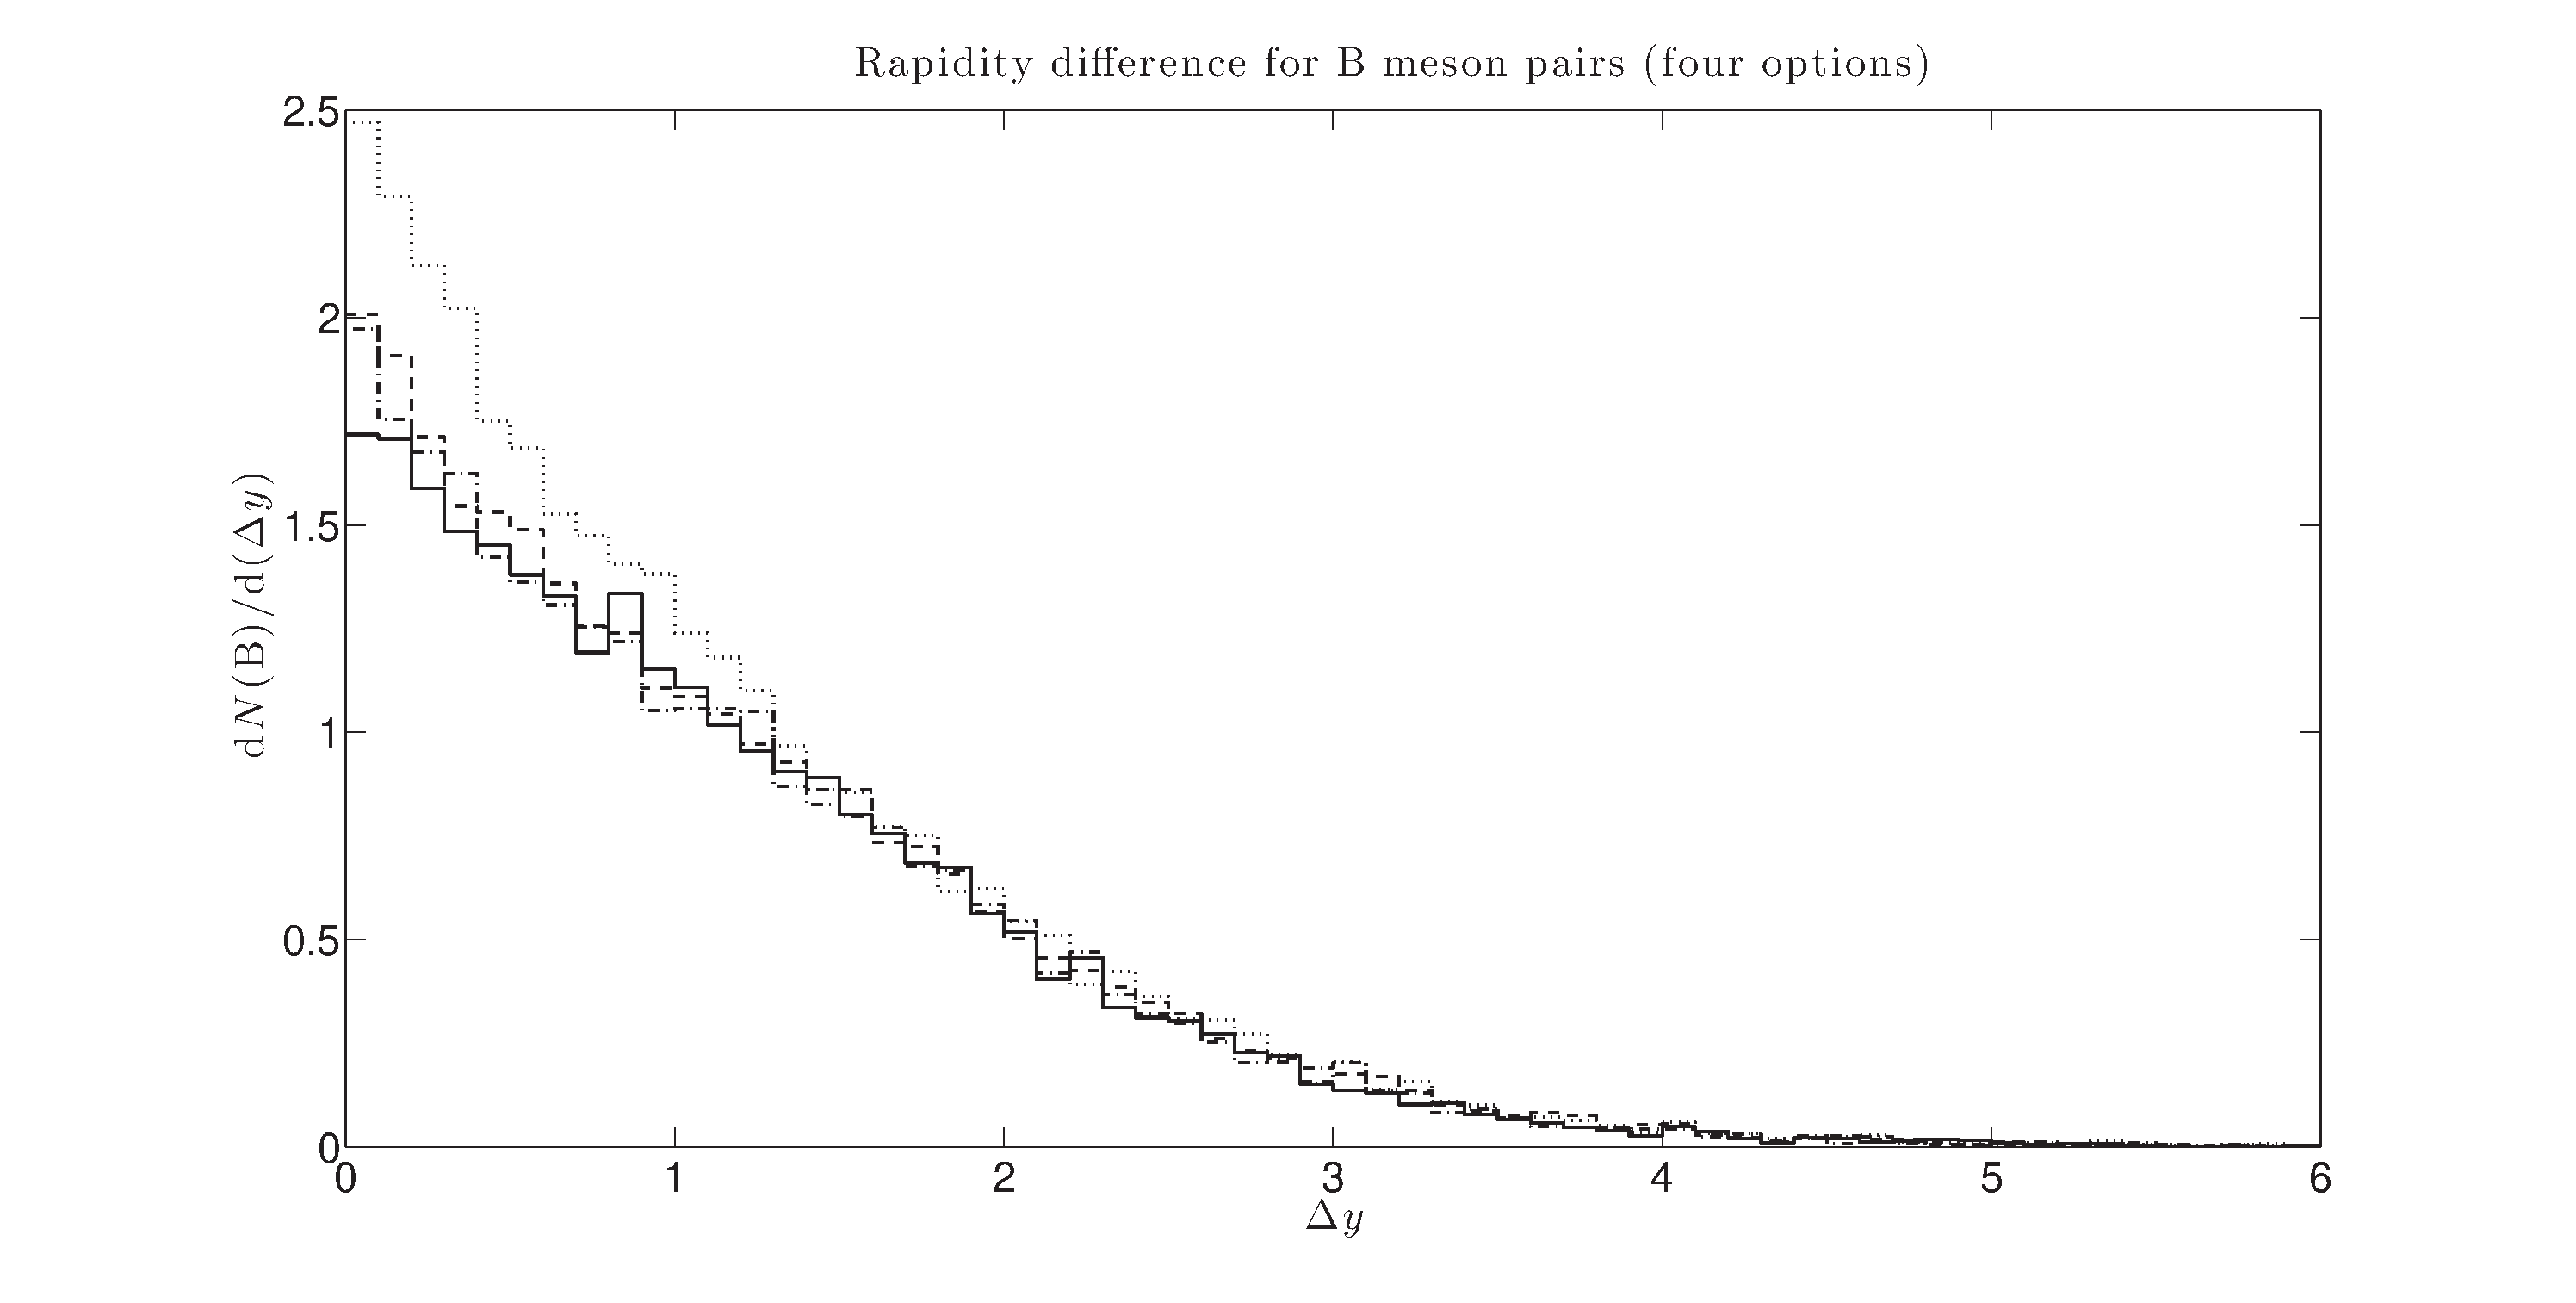
\includegraphics[width=15cm]{BBY4Op.eps}
\label{fig:BBY4Op}
\end{figure}

Low rapiditiy differences mean that the particles in the pairs are close in ``polar distance'', as well as a high $\Delta y$ means a high polar separation. In principle, quarks from PC are produced with a very small rapidity difference, but the kinematical effects of the showering broaden that separation and the corresponding mesons then have a significant contribution at small and medium $\Delta y$ values. On the other hand, the impact of the mesons from GS is mainly at small rapidity differences.

The FE contribution is less important than the one from PC. Flavour excitation falls below GS only at small rapidity differences.

The change in the options is then appreciable at low $\Delta y$ values, whereas in the medium region and in the tail the behaviour is similar for the four options. See fig. \ref{fig:BBY4Op}.

\subsubsection{$R$ distances}

The quantity $R$ contains information from the two variables studied above. In a sense, by giving the $\Delta y$ and $\Delta \varphi$ values of a meson pair, one has a complete (Lorentz invariant to boosts along the $z$-axis) description of the angular distribution for the pair. In the $y - \varphi$ plane, the (also invariant) distance $R=\sqrt{(\Delta y)^2 + (\Delta \varphi)^2}$ is then useful to group the pairs with their angular ``neighbours''. In order to define a \textit{hadron jet}, typically the $R$ distance is used to cluster nearby hadrons.

Figure \ref{fig:BBROp1} shows the behaviour of each source, plus the total production of B mesons for option 1. 
\begin{figure}[!h]
\centering
\caption[$\B$ meson pairs $R$ distances. \textsc{Pythia} default option.]{$R$-distances of $\B$ mesons pairs using \textsc{Pythia} default option, including the four sources.}
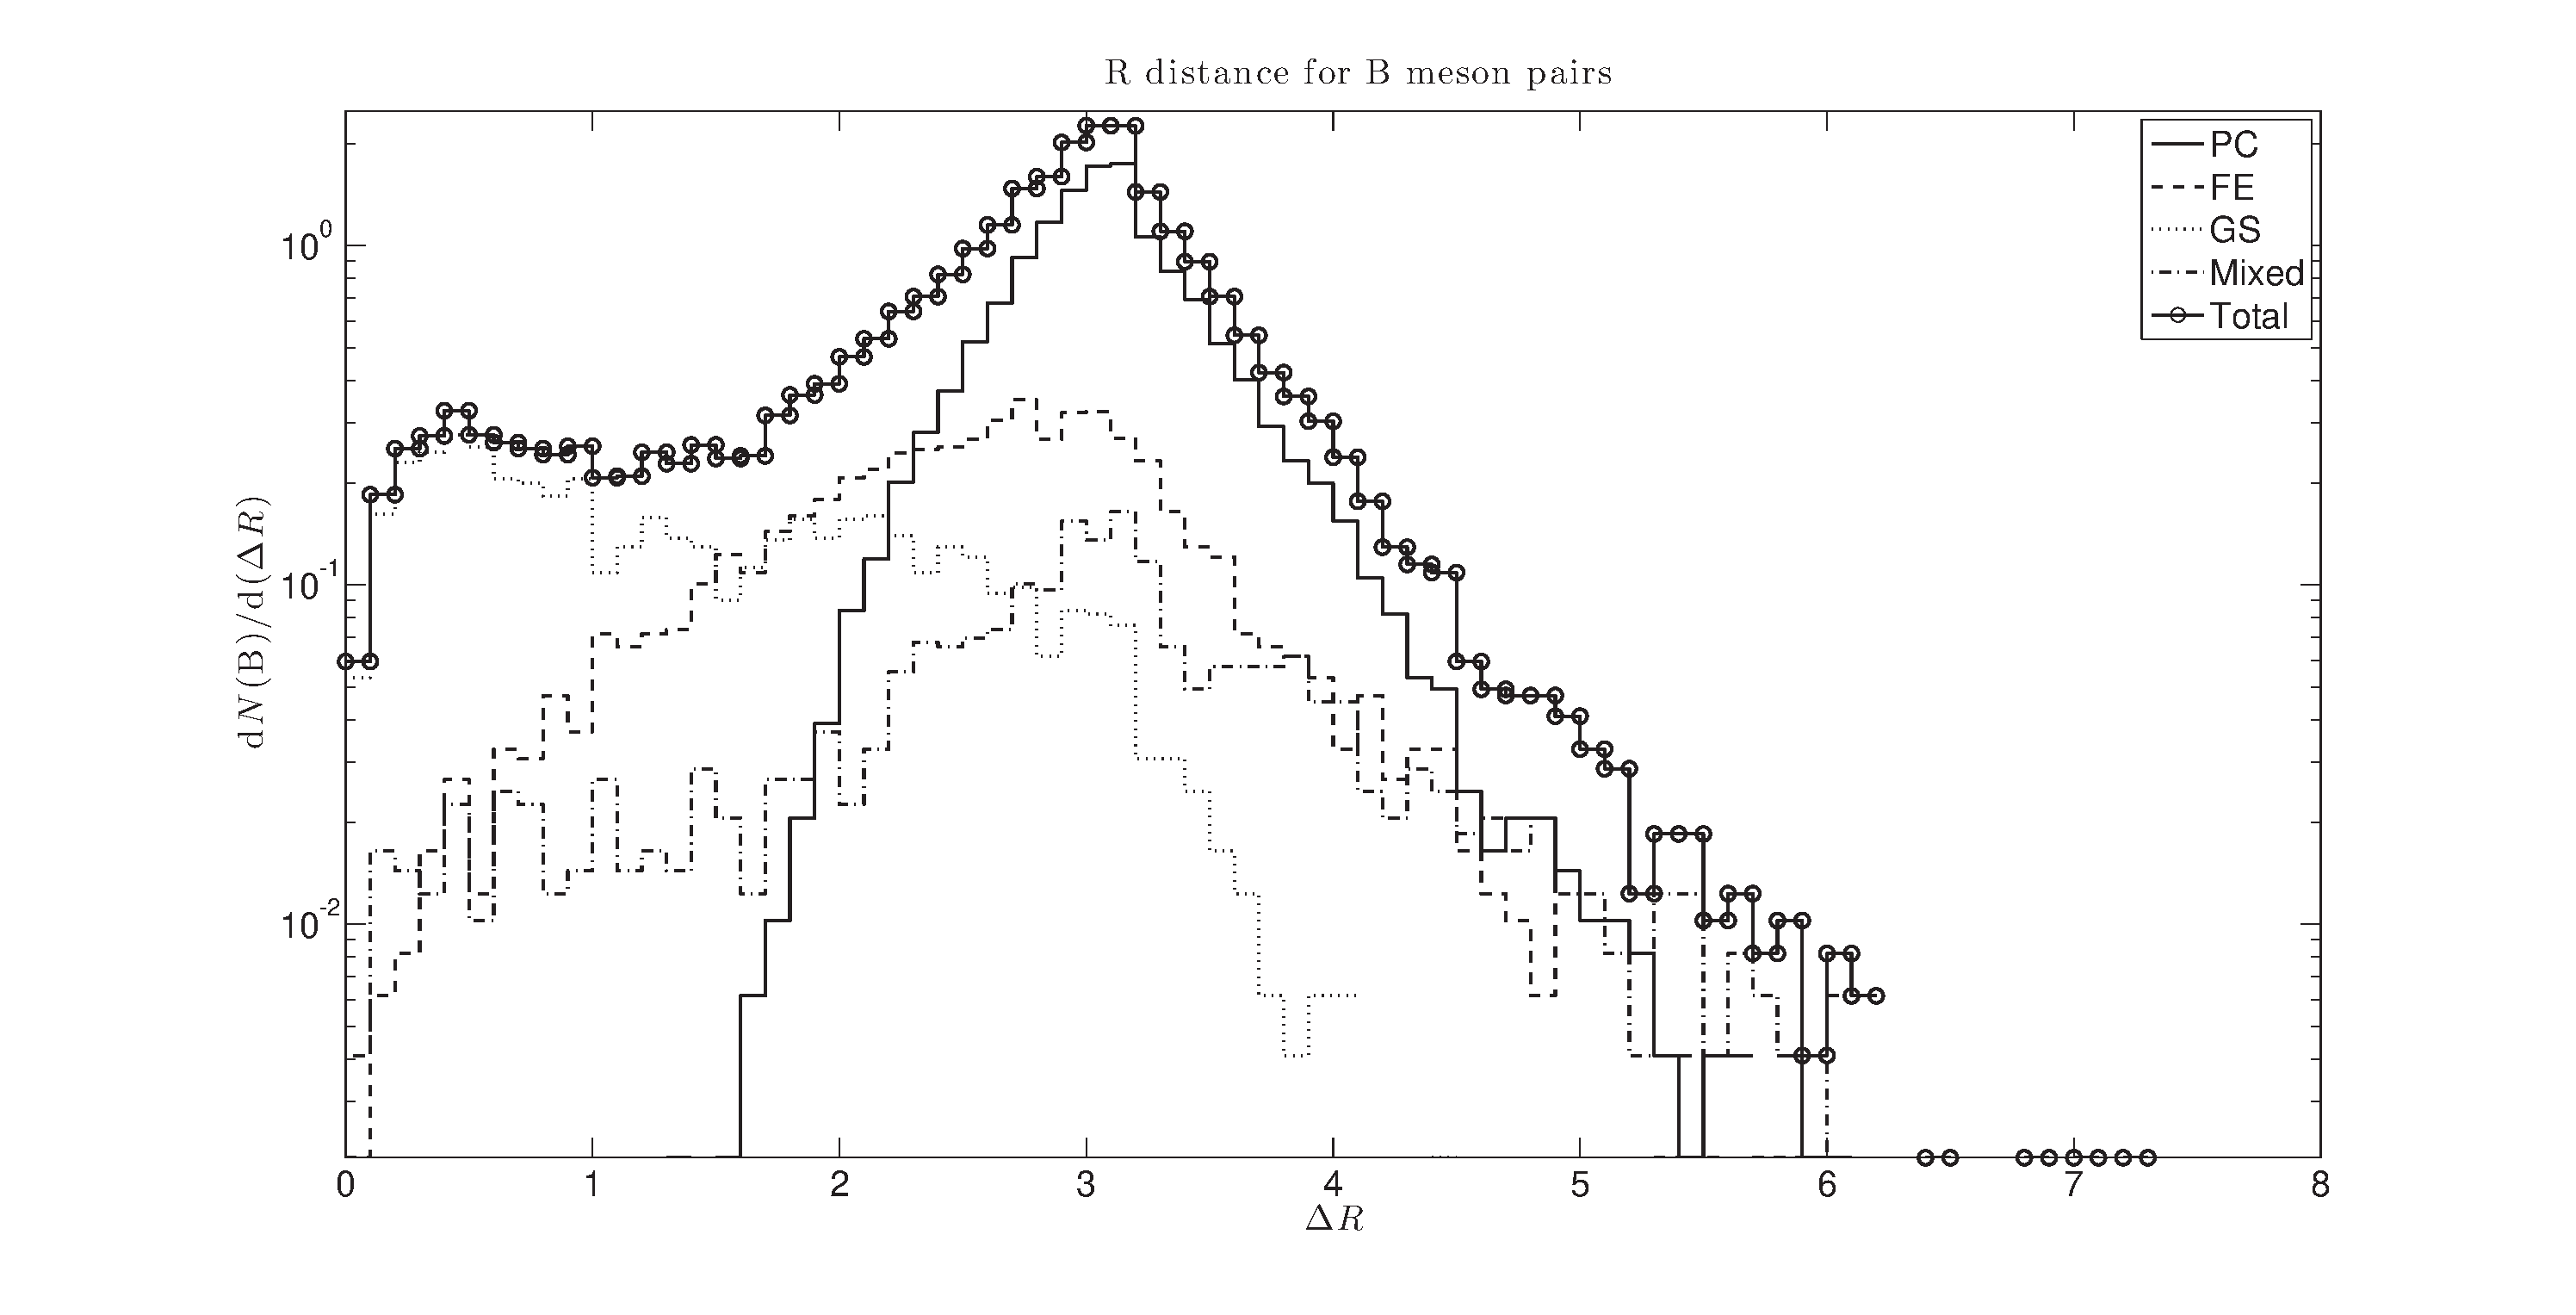
\includegraphics[width=15cm]{BBROp1.eps}
\label{fig:BBROp1}
\end{figure}
Due to the relevant contribution of PC to large azimuthal opening angles, the main peak of the $R$-distance is near to the $\pi$ value. Flavour excitation also presents a growth near that value, but less significant. Mesons produced by means of GS are usually close in both $y$ and $\varphi$ separations, so pairs classified as gluon splitting will be likely to be found in the same jet. 

\begin{figure}[!h]
\centering
\caption[$\B$ meson pairs $R$ distances. Four \textsc{Pythia} options.]{$R$-distances of $\B$ mesons pairs using \textsc{Pythia} options 1 (solid), 2 (dashed), 3 (dotted) and 4 (dashed-dotted).}
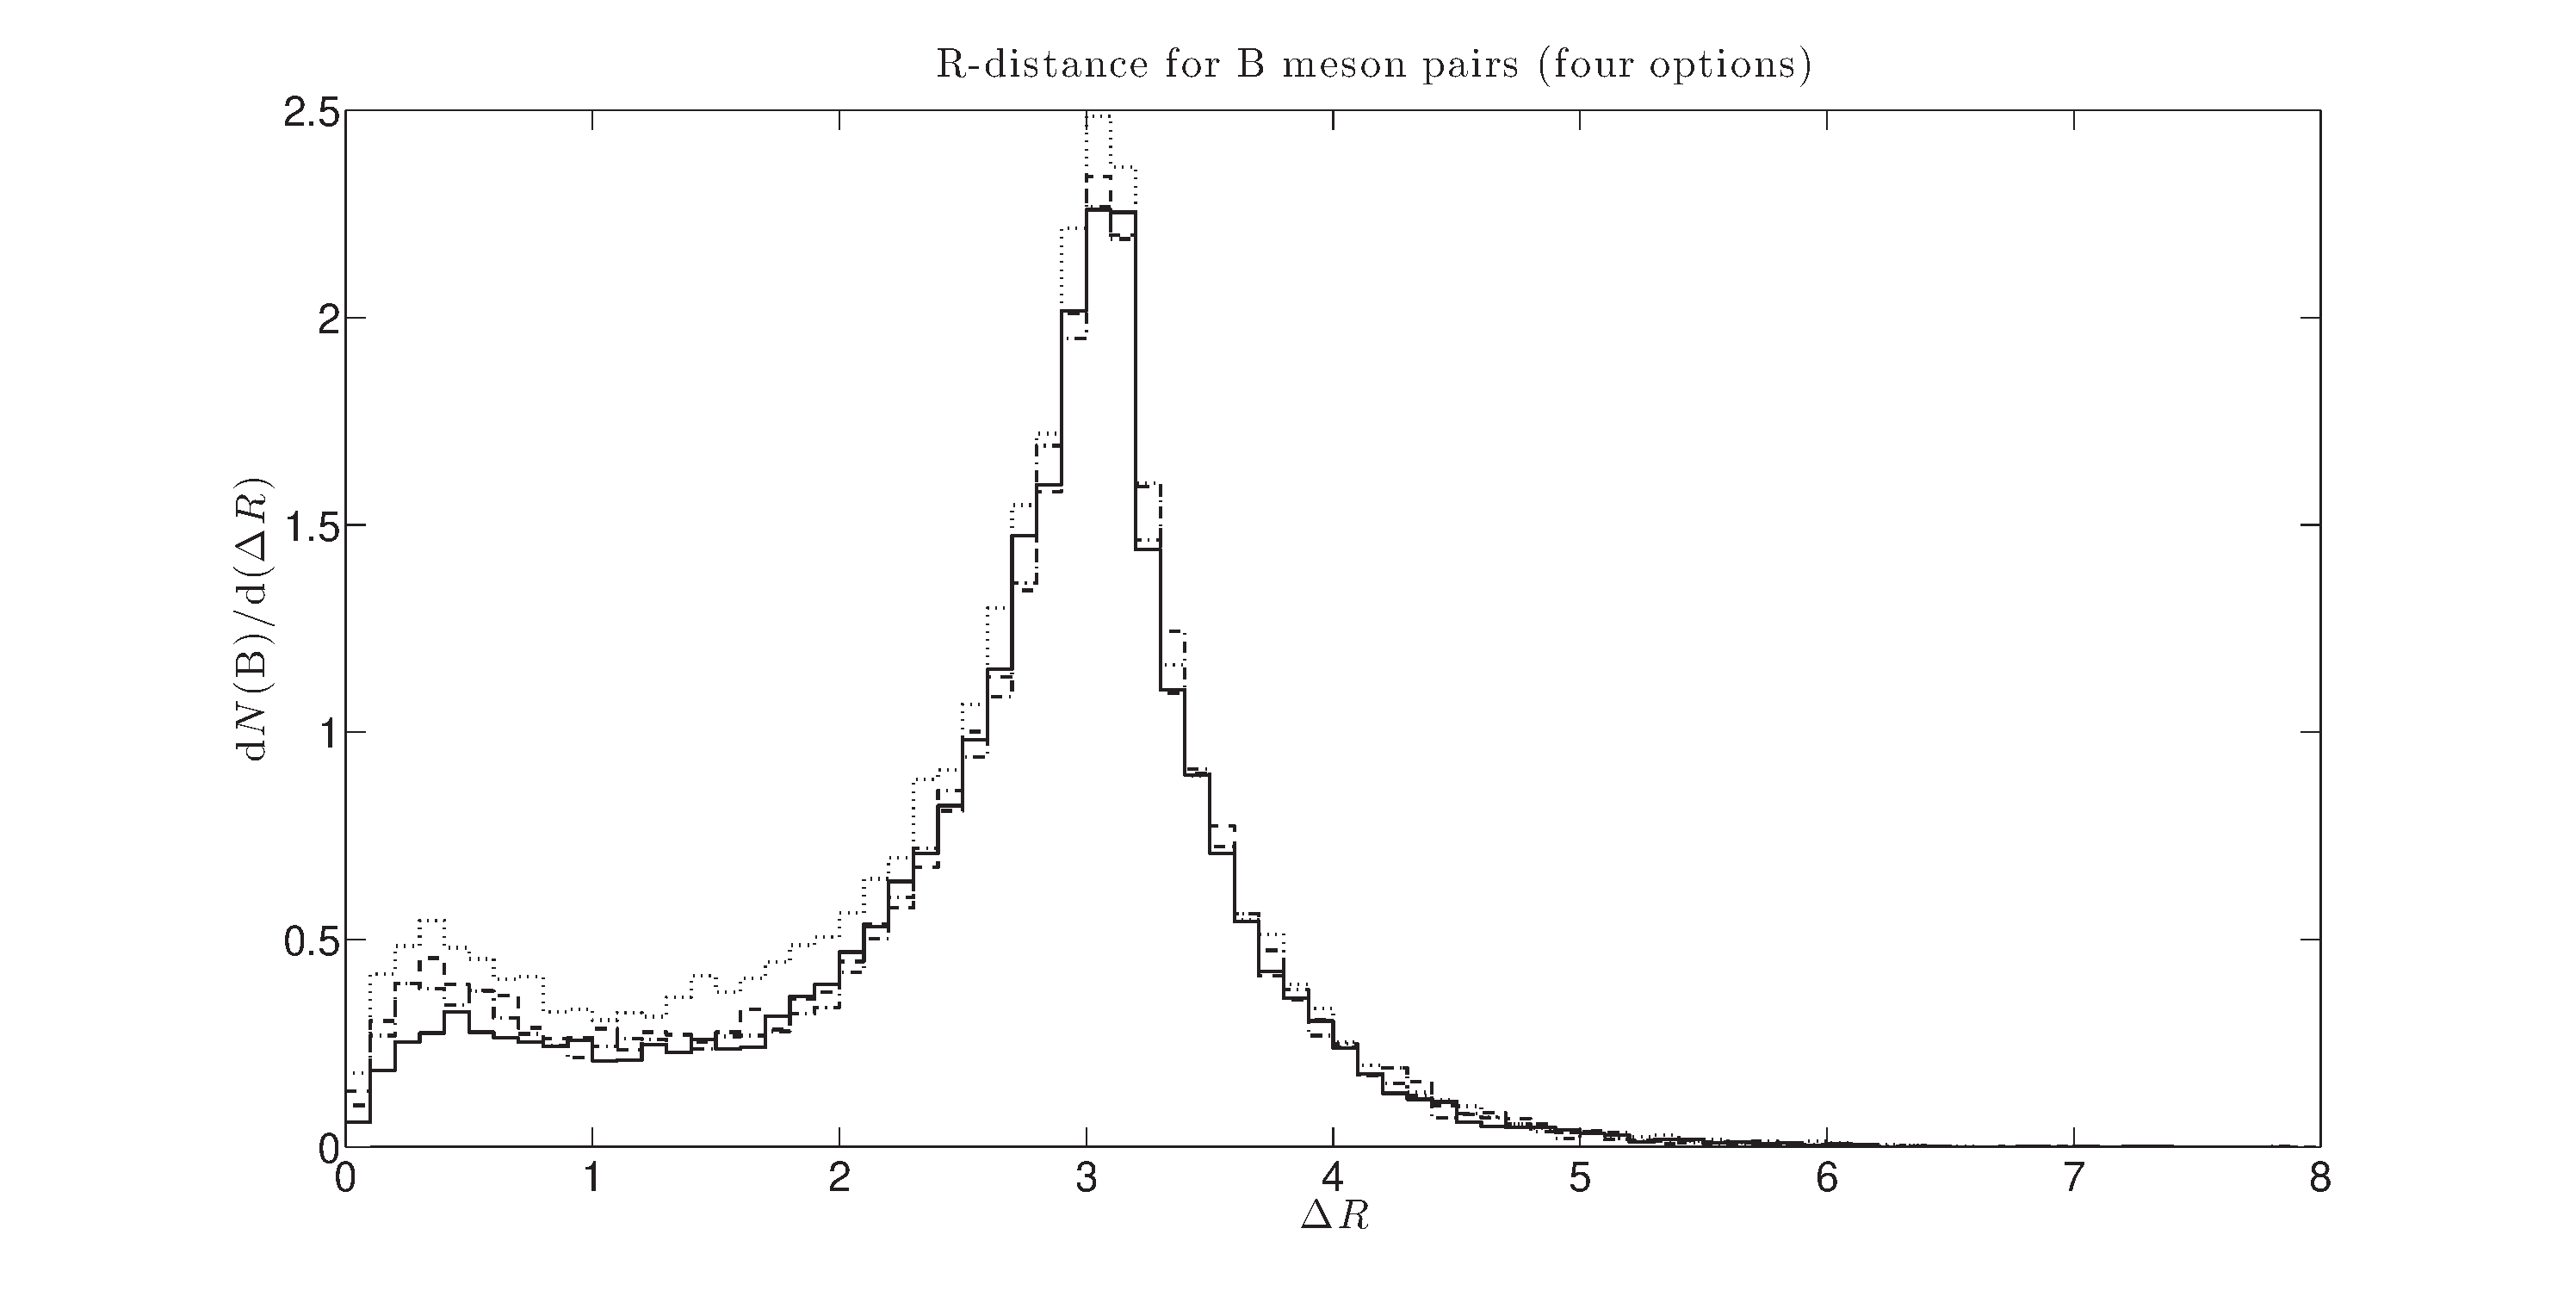
\includegraphics[width=15cm]{BBR4Op.eps}
\label{fig:BBR4Op}
\end{figure}

Since $R$ combines the information from the relative rapidities and the azimuthal angular opening, a respective enhancement is expected for each of the options at small distances, shown in fig. \ref{fig:BBR4Op}.

Experimental data on bottom angular correlations from hadron collisions at the LHC can be found in \cite{Khachatryan:2011wq} and \cite{ATLAS:2011ac}. The analyses done there are included in the set of validation routines provided by Rivet \cite{Buckley:2010ar}. The integration between \textsc{Pythia} and Rivet analyses, and the production of results from it, is a machinery that was considered for this study but not fully implemented due to time constraints. The hadron collision study can also be done for different PDFs, to observe the impact on the production mechanisms and then and compare with experimental data. 

There are also studies on the $\b$ quark production at Tevatron ($\p\pbar$ collisions at 2000 GeV), an example can be found in \cite{vallecorsa}.

\section{Summary and outlook}
\label{sec:summary}

The $\g_{\b\bbar}$ rate was simulated and compared with experimental results. The results agree with the default option implemented in \textsc{Pythia} so far and with option 4 within the experimental error. Remarkably, the enhancement introduced by option 4 at the mass threshold region is almost exactly canceled by the suppression at high masses, leading to a rate close to the default. Option 2 gives a result within two standard deviations compared to experimental data, whereas option 3 does not seem to reproduce the rate at all. Options 5-8, using $m^2$ as the argument of the strong coupling, do not affect sensibly the rate (around 5\% difference for each option).

A limited set of data is available for the study of heavy quarks at lepton collisions. A future measurement of the production of heavy quarks as a function of the invariant mass of the pairs could shed light on which of the options is more suitable, or the need for a new one.

The study is inconclusive regarding the $\D^{*\pm}$ energy spectrum. The default option shows a deficiency for low energy fractions that could be corrected by the enhancement given by the alternative options, particularly option 3. However, all the options present an excess at the medium region that, if shifted back to the low region by e.g a different modeling of the $\B\to\D$ decay, could also reconcile \textsc{Pythia}  and the data, without introducing a higher $\g\to\Q\Qbar$ rate.

For proton-proton collisions at typical LHC energies the azimuthal angular openings, the relative rapidities and the $R$ distances of $\B$ meson pairs were simulated. The contributions of the production mechanisms to the mentioned quantities are shown. The variation of the observables using the four \textsc{Pythia} options is also shown. Using transverse momentum lower cutoffs for the generation of the events and for the analyzed $\B$ mesons, the selected events were around 1.5\% of the generated ones.

Further studies could begin by comparing the simulated results for the four options with data. There exist experimental results and analyses for Tevatron and LHC experiments, based on different event reconstruction mechanisms. The dependence of the correlations and the production rates implementing different PDFs could also be explored in this context. 

\section*{Acknowledgements}

I would like to thank Torbjörn Sjöstrand for his patient advisement and corrections to the earlier versions of this work. The valuable discussions with him were essential for the developing of the ideas presented here. I am also grateful to my family and friends, who have supported me during my stay in Sweden.

\clearpage
\begin{thebibliography}{99}


%\cite{Sjostrand:2006za}
\bibitem{Sjostrand:2006za}
  T.~Sjöstrand, S.~Mrenna and P.~Z.~Skands,
  %``PYTHIA 6.4 Physics and Manual,''
  JHEP {\bf 0605} (2006) 026
  [hep-ph/0603175].
  %%CITATION = HEP-PH/0603175;%%
  %5087 citations counted in INSPIRE as of 28 Apr 2014

%\cite{Sjostrand:2007gs}
\bibitem{Sjostrand:2007gs}
  T.~Sjöstrand, S.~Mrenna and P.~Z.~Skands,
  %``A Brief Introduction to PYTHIA 8.1,''
  Comput.\ Phys.\ Commun.\  {\bf 178} (2008) 852
  [arXiv:0710.3820 [hep-ph]].
  %%CITATION = ARXIV:0710.3820;%%
  %1065 citations counted in INSPIRE as of 28 Apr 2014
  
%\cite{Beringer:1900zz}
\bibitem{Beringer:1900zz}
  J.~Beringer {\it et al.}  [Particle Data Group Collaboration],
  %``Review of Particle Physics (RPP),''
  Phys.\ Rev.\ D {\bf 86} (2012) 010001.
  %%CITATION = PHRVA,D86,010001;%%
  %3768 citations counted in INSPIRE as of 29 Apr 2014  

%\cite{Kane:1993}
\bibitem{Kane:1993}
 G.~Kane,
 ``Modern elementary particle physics: the fundamental particles and forces?,''
 Perseus publishing (1993).
 %%CITATION = HPACA,25,417;%%

%\cite{Peskin:1995} 
\bibitem{Peskin:1995}
  M.~E.~Peskin and D.~V.~Schroeder,
  ``An Introduction To Quantum Field Theory,''
%\href{http://www.slac.stanford.edu/spires/find/hep/www?irn=3485960}{SPIRES entry}
{\it  Reading, USA: Addison-Wesley (1995) 842 p}.

%\cite{Sjostrand:2009ad}
\bibitem{Sjostrand:2009ad}
  T.~Sjöstrand,
  %``Monte Carlo Tools,''
  arXiv:0911.5286 [hep-ph].
  %%CITATION = ARXIV:0911.5286;%%
  %11 citations counted in INSPIRE as of 28 Apr 2014

%\cite{Boos:2001cv}
\bibitem{Boos:2001cv}
  E.~Boos, M.~Dobbs, W.~Giele, I.~Hinchliffe, J.~Huston, V.~Ilyin, J.~Kanzaki and K.~Kato {\it et al.},
  %``Generic user process interface for event generators,''
  hep-ph/0109068.
  %%CITATION = HEP-PH/0109068;%%
  %175 citations counted in INSPIRE as of 21 Jun 2014

% The next five articles correspond to the measurement of the g_{bb} rate.
%\cite{Abreu:1997nf} \cite{Barate:1998vs} \cite{Abe:1999qg} \cite{Abreu:1999qh} \cite{Abbiendi:2000zt}

% \cite{Abreu:1997nf}
\bibitem{Abreu:1997nf}
  P.~Abreu {\it et al.}  [DELPHI Collaboration],
  %``Measurement of the multiplicity of gluons splitting to bottom quark pairs in hadronic Z0 decays,''
  Phys.\ Lett.\ B {\bf 405} (1997) 202.
  %%CITATION = PHLTA,B405,202;%%
  %45 citations counted in INSPIRE as of 15 May 2014
  
%\cite{Barate:1998vs}
\bibitem{Barate:1998vs}
  R.~Barate {\it et al.}  [ALEPH Collaboration],
  %``A Measurement of the gluon splitting rate into b anti-b pairs in hadronic Z decays,''
  Phys.\ Lett.\ B {\bf 434} (1998) 437.
  %%CITATION = PHLTA,B434,437;%%
  %42 citations counted in INSPIRE as of 15 May 2014
  
%\cite{Abe:1999qg}
\bibitem{Abe:1999qg}
  K.~Abe {\it et al.}  [SLD Collaboration],
  %``Measurement of the probability for gluon splitting into b anti-b in Z0 decays,''
  hep-ex/9908028.
  %%CITATION = HEP-EX/9908028;%%
  %8 citations counted in INSPIRE as of 15 May 2014
  
%\cite{Abreu:1999qh}
\bibitem{Abreu:1999qh}
  P.~Abreu {\it et al.}  [DELPHI Collaboration],
  %``Measurement of the rate of b anti-b b anti-b events in hadronic Z decays and the extraction of the gluon splitting into b anti-b,''
  Phys.\ Lett.\ B {\bf 462} (1999) 425.
  %%CITATION = PHLTA,B462,425;%%
  %27 citations counted in INSPIRE as of 15 May 2014

%\cite{Abbiendi:2000zt}
\bibitem{Abbiendi:2000zt}
  G.~Abbiendi {\it et al.}  [OPAL Collaboration],
  %``Production rates of b anti-b quark pairs from gluons and b anti-b b anti-b events in hadronic Z0 decays,''
  Eur.\ Phys.\ J.\ C {\bf 18} (2001) 447
  [hep-ex/0010029].
  %%CITATION = HEP-EX/0010029;%%
  %16 citations counted in INSPIRE as of 19 May 2014

%\cite{Barate:1999bg}
\bibitem{Barate:1999bg}
  R.~Barate {\it et al.}  [ALEPH Collaboration],
  %``Study of charm production in Z decays,''
  Eur.\ Phys.\ J.\ C {\bf 16} (2000) 597
  [hep-ex/9909032].
  %%CITATION = HEP-EX/9909032;%%
  %123 citations counted in INSPIRE as of 11 May 2014
  
%\cite{Norrbin:2000zc}
\bibitem{Norrbin:2000zc}
  E.~Norrbin and T.~Sjöstrand,
  %``Production and hadronization of heavy quarks,''
  Eur.\ Phys.\ J.\ C {\bf 17} (2000) 137
  [hep-ph/0005110].
  %%CITATION = HEP-PH/0005110;%%
  %113 citations counted in INSPIRE as of 12 May 2014

%\cite{Khachatryan:2011wq} \cite{ATLAS:2011ac}
\bibitem{Khachatryan:2011wq}
  V.~Khachatryan {\it et al.}  [CMS Collaboration],
  %``Measurement of $B\bar{B}$ Angular Correlations based on Secondary Vertex Reconstruction at $\sqrt{s}=7$ TeV,''
  JHEP {\bf 1103} (2011) 136
  [arXiv:1102.3194 [hep-ex]].
  %%CITATION = ARXIV:1102.3194;%%
  %50 citations counted in INSPIRE as of 26 May 2014

%\cite{ATLAS:2011ac}
\bibitem{ATLAS:2011ac}
  G.~Aad {\it et al.}  [ATLAS Collaboration],
  %``Measurement of the inclusive and dijet cross-sections of $b^-$ jets in $pp$ collisions at $\sqrt{s}=7$ TeV with the ATLAS detector,''
  Eur.\ Phys.\ J.\ C {\bf 71} (2011) 1846
  [arXiv:1109.6833 [hep-ex]].
  %%CITATION = ARXIV:1109.6833;%%
  %41 citations counted in INSPIRE as of 26 May 2014

%\cite{Buckley:2010ar}
\bibitem{Buckley:2010ar}
  A.~Buckley, J.~Butterworth, L.~Lonnblad, D.~Grellscheid, H.~Hoeth, J.~Monk, H.~Schulz and F.~Siegert,
  %``Rivet user manual,''
  Comput.\ Phys.\ Commun.\  {\bf 184} (2013) 2803
  [arXiv:1003.0694 [hep-ph]].
  %%CITATION = ARXIV:1003.0694;%%
  %137 citations counted in INSPIRE as of 21 Jun 2014

%\cite{vallecorsa}
\bibitem{vallecorsa}
  S. Vallecorsa,
  ``Measurement of the $\b\bbar$ di-jet cross section at CDF,''
  Univ. of Geneva Thesis (2007) 3916.

\end{thebibliography}

%\includegraphics[width=8cm]{Draco_cmd.ps}

\end{document}